\chapter{High Voltage System}
\label{ch:fdsp-hv}

%%%%%%%%%%%%%%%%%%%%%%%%%%%%%%%%%%%%%%%%%%%%%%%%%%%%%%%%%%%%%%%%%%%%
\section{High Voltage System (HV) Overview}
\label{sec:fdsp-hv-ov}


%%%%%%%%%%%%%%%%%%%%%%%%%%%%%%%%%
\subsection{Introduction}
\label{sec:fdsp-hv-intro}
A liquid argon cryostat requires an equipotential cathode plane of high voltage (CPA-Plane), and a precisely regulated interior electric field to drive electrons from particle interactions to the sensor planes (APA's, see volume 3A). In the case of the DUNE Single Phase (SP) detector, this requires vertical CPA-Planes held at high voltage, and formed sets of conductors at graded voltages on the top and bottom (Field Cages, or FC's) and sides (Endwall Filed Cages, or EW-FC's) of the central drift volume.

The modular TPC construction is shown in fig \ref{fig:dune_sp_fd}. A DUNE TPC is made up of 25 such assemblies, plus two complete end wall field cage planes, with the  drift fields transporting the ionization electrons in the direction CPA $\Rightarrow$ APA. 

\begin{dunefigure}[One unit of DUNE showing CPAs, and APAs]{fig:dune_sp_fd}
{Interior of DUNE SP TPC. The CPA's occupy the 2nd and 4th positions, between 3 APA's. Top and bottom field cages are shown in blue(Credit: CAD model)}
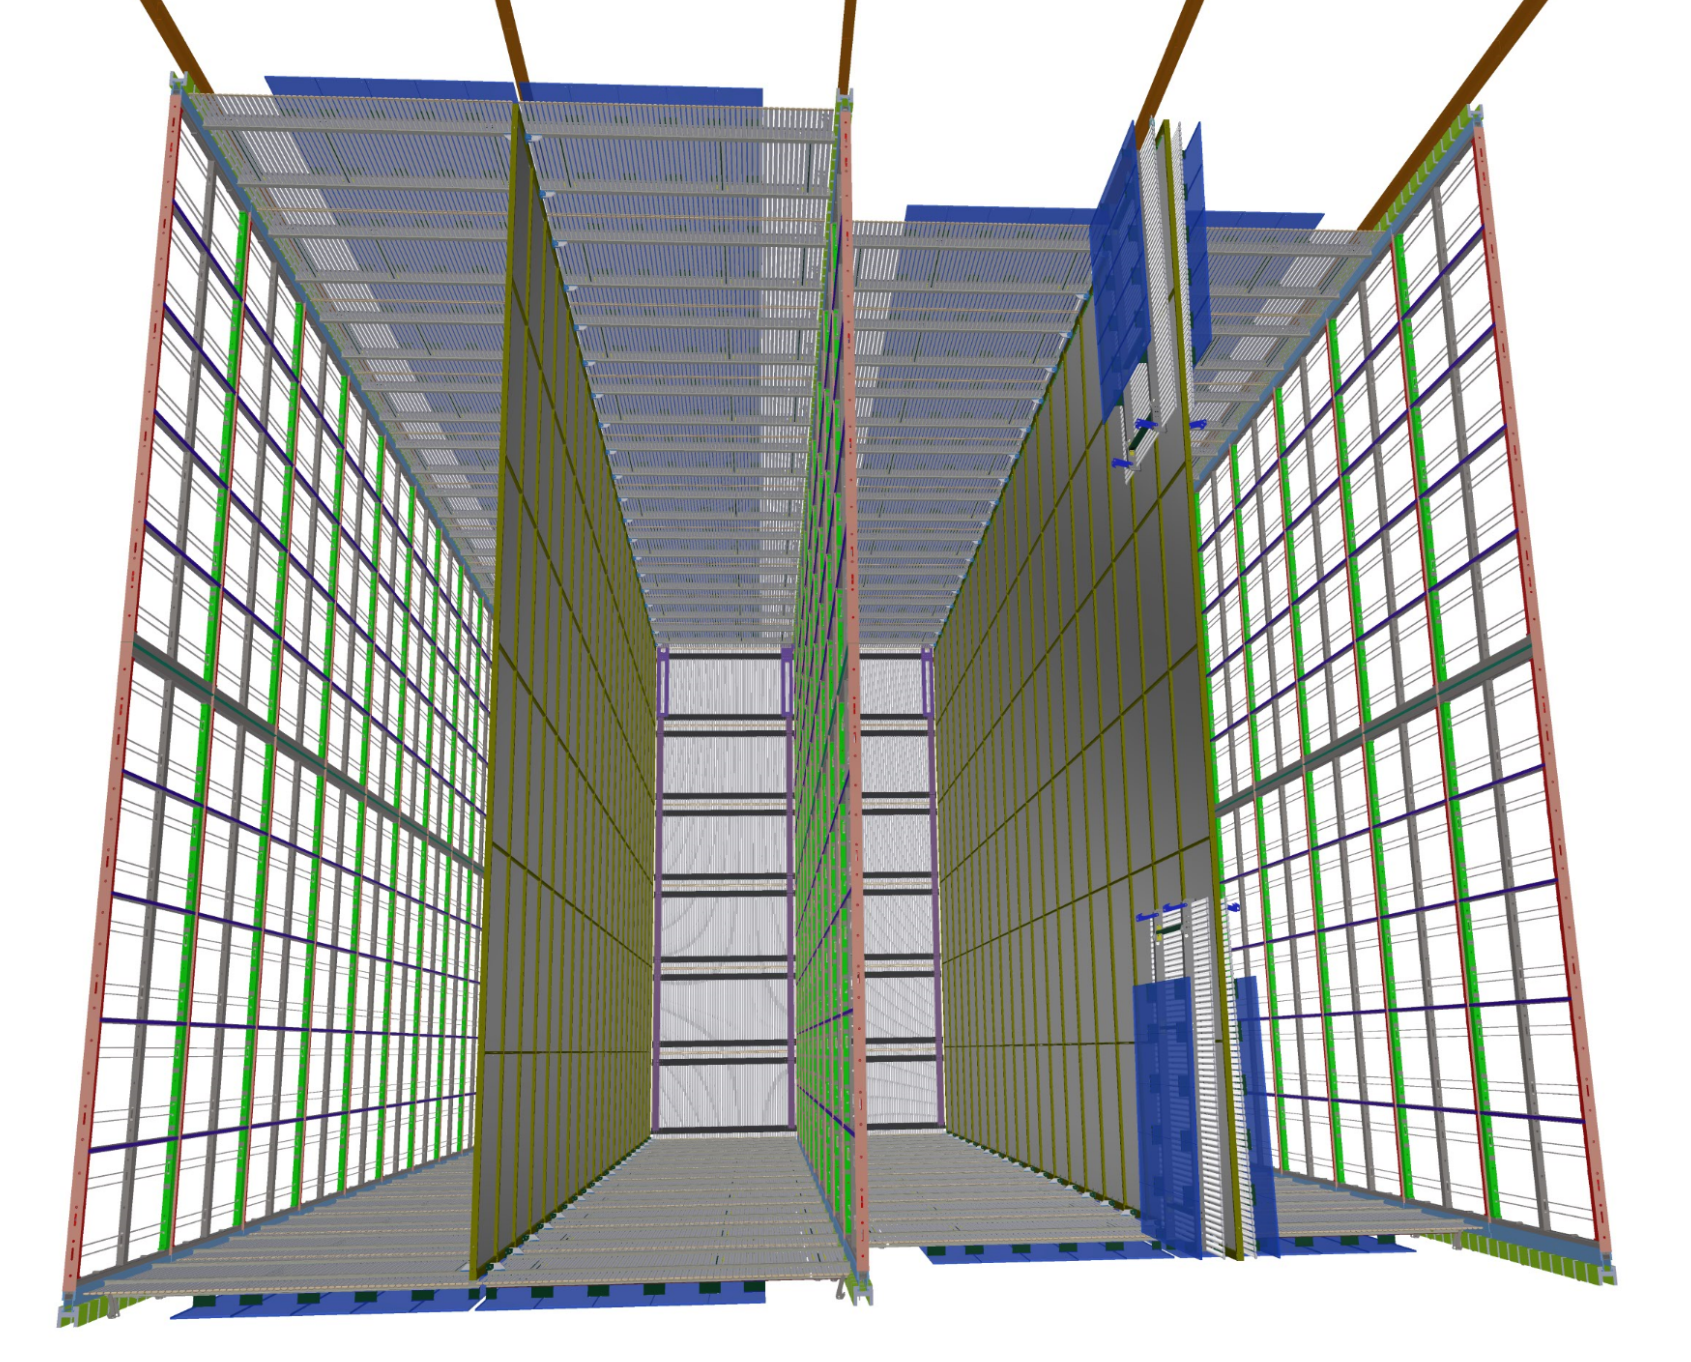
\includegraphics[width=0.8\textwidth]{dune_sp_fd}
\end{dunefigure}
%\begin{dunefigure}[One unit of DUNE showing CPA's,  and APA's]{fig:HV_Module}
%{One unit of DUNE showing CPA's and APA's. The CPA's occupy the 2nd and 4th positions, between 3 APA's. Top and bottom field cages are shown in blue(Credit: CAD model)}
%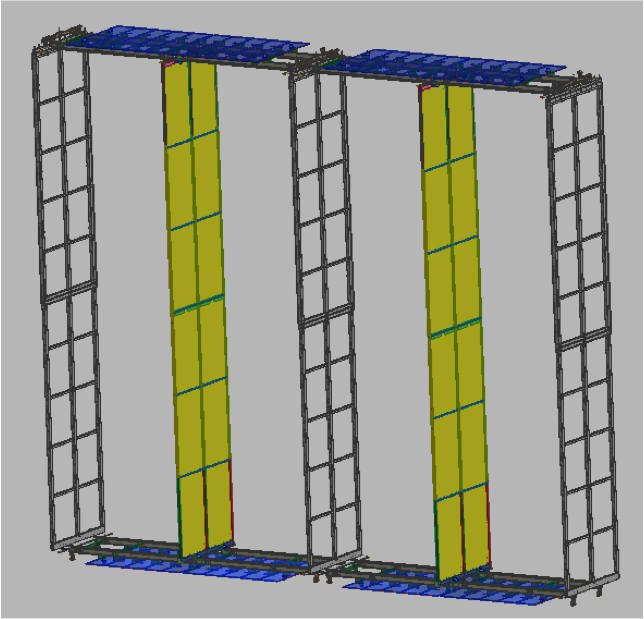
\includegraphics[width=0.5\textwidth]{HV_Module.png}
%\end{dunefigure}

It is to be noted that the HV Consortium provides systems that operate at all voltages from the highest to ground inside the TPC volume. As a result its systems actually constitute a large fraction of the total internal structures of the TPC itself, the principal exception being the APA's and Photon Detectors (PD's). Mechanical and structural concerns will work together with electrical design to meet the requirements.

%%%%%%%%%%%%%%%%%%%%%%%%%%%%%%%%%%%%%
\subsection{Design Requirements}
\label{sec:fdsp-hv-des-consid}
 
The TPC HV System is designed to meet the Physics Requirements of the DUNE Experiment. These are both physical requirements (such as electric fields that allow robust event reconstruction) and operational (a system that avoids over-complication so as to maximize the time that the detector can collect neutrino events). An important collection of the requirements is shown in Table ~\ref{tab:hvphysicsreqs}.


\begin{dunetable}
[HV System Requirements]
{p{0.2\linewidth}p{0.4\linewidth}p{0.15\linewidth}p{0.15\linewidth}}
{tab:hvphysicsreqs}
{HV System Requirements}   
 Requirement & Physics Requirement Driver & Requirement & Goal \\ \toprowrule
Exceed minimum electric field in TPC drift volume & Maintain adequate particle ID, which is impacted by slower drift speed and increased recombination, diffusion and space charge effects. & >250 v/cm &500 V/cm \\ \colhline
  Do not exceed maximum electric field in LAr volume & Avoid damage to detector to enable data collection over long periods. & 30 kV/cm & @ ALARA \\  \colhline
 Minimize power supply ripple & Keep readout electronics free from external noise, which confuses event reconstruction.  \\ \colhline
 Maximize power supply stability & Maintain the ability to reconstruct data taken over long period.  Maintain high operational uptime to maximize experimental statistics. \\ \colhline
 Provide adequate decay constant for discharge of the cathode surface and field cage  & Avoid damage to detector to enable data collection over long periods. Maintain high operational uptime to maximize experimental statistics. & MOhm/square & GOhm/square \\ \colhline
 Provide redundancy in all HV connections & Avoid single point failures in detector which interrupt datataking.\\ 
\end{dunetable}


%%%%%%%%%%%%%%%%%%%%%%%%%%%%%%%%
\subsection{Scope}
\label{sec:fdsp-hv-scope}

This section discusses the  scope of the HV system, which includes the selection and procurement of materials for, and the fabrication, testing, delivery and installation of systems to generate, distribute, and regulate voltages which create a precision electric field within the DUNE detector volume. 

The HV system consists of components both exterior and interior to the cryostat. The HV power supplies and filters pass through the HV feedthrough and are further distributed by components which form part of the TPC structure. These are:
\begin{itemize}
\item Power Supply
\item Cathode Plane
\item Top and Bottom Field Cages and Ground Planes
\item Endwall Field Cages 
\end{itemize}
The TPC has a 2 central Cathode Plane Arrays (CPA-arrays), 57.5m long and 12m tall, with two symmetric drift volumes on both sides. There are 25 CPA-planes in each CPA-array, installed contiguously along the length of the TPC. A CPA-plane is assembled from 2 side-by-side Cathode Plane Assembly Panel (CPA-panels). Each CPA-panel is 1.2m in width and 12m tall, formed from 3 vertically stacked CPA-Units, and supported from above by the CPA installation rail, through a single link.
A CPA-Unit consists of a FR4 frame that encloses and supports its resistive panels.  Each CPA-Unit is approximately 1.2m wide and 4m high and is constructed from two resistive panel modules.

The sides of the drift volumes on both sides of the CPA-plane are covered by the FC and EW field cage modules to define a uniform drift field of 500V/cm, with a increasing potential over 3.6m from the high voltage CPA (-180kV) to ground potential at the APA sensor planes, . The cathode bias is provided by an external high voltage power supply through an HV feedthrough connecting to the CPA-plane inside the cryostat.
The Field Cage modules have two distinctive types: the top/bottom (FC), which run the full length of the detector, and the end walls (EW's), which complete the detector at either end. The modules of both systems are constructed from an array of extruded aluminum open profiles supported by FRP (fiber reinforced plastic) structural beams. A resistive divider chain interconnects all the metal profiles to provide a linear voltage gradient between the cathode and anode planes.  The top/bottom modules are nominally 2.3m wide by 3.6m long. 

A ground plane of tiled perforated stainless steel sheet panels is mounted on the outside surface of each of the top/bottom field cage modules with a 20cm clearance. The top and bottom  FC modules are supported by the CPA's and APA's. The end wall modules are 1.5m tall by 3.6m long. They are stacked 8 units high to cover the 12m height of the TPC.  These EW-FC modules are supported by the installation rails above  the APA's and CPA's, which are part of the Detector Support Structure (DSS). 

For ease of understanding the rather complex physical layout of the systems comprising the HV and electric field hardware, Tables ~\ref{tab:cpaparts} and ~\ref{tab:fcparts} contain summaries of terminology and parts.

\begin{dunetable}
[HV Cathode Plane Components]
{p{0.37\linewidth}p{0.07\linewidth}p{0.07\linewidth}p{0.07\linewidth}p{0.07\linewidth}
p{0.1\linewidth}p{0.15\linewidth}}
{tab:cpaparts}
{HV Cathode Plane Components} 
Component & Count & Length (z) & Width (x) & Height (y) & Submodules & Grand Total \\ \toprowrule
CPA-Array & 2 & 57.5 m & - & 12 m & 25 & 2 \\ \colhline
CPA-Plane (per CPA-Array) & 25 & 2.3 m & - & 12 m & 2 & 50 \\ \colhline
CPA-Panel (per CPA-Plane) & 2 & 1.2 m & - & 12 m & 3 & 100 \\ \colhline
CPA-Unit (per CPA-Panel) & 3 & 1.2 m & - & 4 m & 2 & 300 \\ \colhline
CPA-RP (per CPA-Unit) & 2 & 1.2 m & - & 2 m & - & 600 \\
\end{dunetable}

\begin{dunetable}
[HV Field Cage Components]
{p{0.37\linewidth}p{0.07\linewidth}p{0.07\linewidth}p{0.07\linewidth}p{0.07\linewidth}
p{0.1\linewidth}p{0.15\linewidth}}
{tab:fcparts}{HV Field Cage Components}
Component & Count & Length (z) & Width (x) & Height (y) & Submodules & Grand Total \\ \toprowrule
FC (Top/Bottom Field Cage) & 200 & 2.3 m & 3.6 m & - & 57 & 200 \\ \colhline
FC-Profiles (per FC) & 57 & 2.3 m & - & - & - & 11400 \\ \colhline
Ground Plane Modules (per FC) & 5 & 2.3 m & 0.7 m & - & - & 1000 \\ \colhline
EW-Plane (Endwall Field Cage) & 2 & - & 14.4 m & 12 m & 4 & 2 \\ \colhline
EW (per EW-Plane) & 4 & - & 3.6 m & 12 m & 8 & 8 \\ \colhline
EW-Modules (per EW) & 8 & - & 3.6 m & 1.5 m & 57 & 64 \\ \colhline
EW-Profiles (per EW-Module) & 57 & - & - & 1.5 m & - & 3648 \\
\end{dunetable}
%%%%%%%%%%%%%%%%%%%%%%%%%%%%%%%%%%%%%%%%%%%%%%%%%%%%%%%%%%%%%%%%%%%%
\section{HV System Design}
\label{sec:fdsp-hv-design}

\subsection {High Voltage Power Supply and Feedthrough (Sarah)}
The HV delivery system consists of
\begin{itemize}
\item Two power supplies.
\item HV cables.
\item Filter resistors.
\item HV feedthroughs into the cryostat.
\end{itemize}

For high voltage delivery, two power supplies will be used to generate the voltage, one for each CPA-Array. This separated setup more easily accommodates different running conditions and helps isolate any instabilities.  In the event only one power supply is available, the system will be run by using a high voltage splitter outside of the cryostat while another power supply is procured. In addition, the cryostat design has 2 feedthrough ports for each CPA-Array, one at each end of the cryostat. The unequipped, downstream port provides redundancy against any failure of the primary HV delivery system.

The planned power supply model, for the SP TPC, will be similar to the Heinzinger PNChp 200000 (used on ProtoDUNE) with a maximum output voltage of \SI{200}{kV} and a maximum current draw of \SI{0.5}{mA}.  An additional option is an existing \SI{300}{kV} \SI{0.5}{mA} model. 

%The high voltage cables will be either Dielectric Sciences model number 2134 capable of \SI{200}{kV} DC or 2236 capable of \SI{320}{kV} DC. 
%ielectrThe high voltage cables are preferred to be Dielectric Sciences model number 2134 capable of \SI{200}{kV} DC.  A back up plan is to use model 2236 capable of \SI{320}{kV} DC. 

The high voltage cables will be commercially available models compatible with the selected power supplies. 

An example schematic is shown in Figure~\ref{fig:ps_filter_ft_schematic}.

\begin{dunefigure}[A schematic showing the high voltage delivery system to the cryostat.  The two filters are places such that one is near the power supply and one is near the feedthrough.]{fig:ps_filter_ft_schematic}
{Left:  A schematic showing the high voltage delivery system to the cryostat.  The two filters are places such that one is near the power supply and one is near the feedthrough. Right:  An example Heinzinger power supply.  (Credit: SEL)}
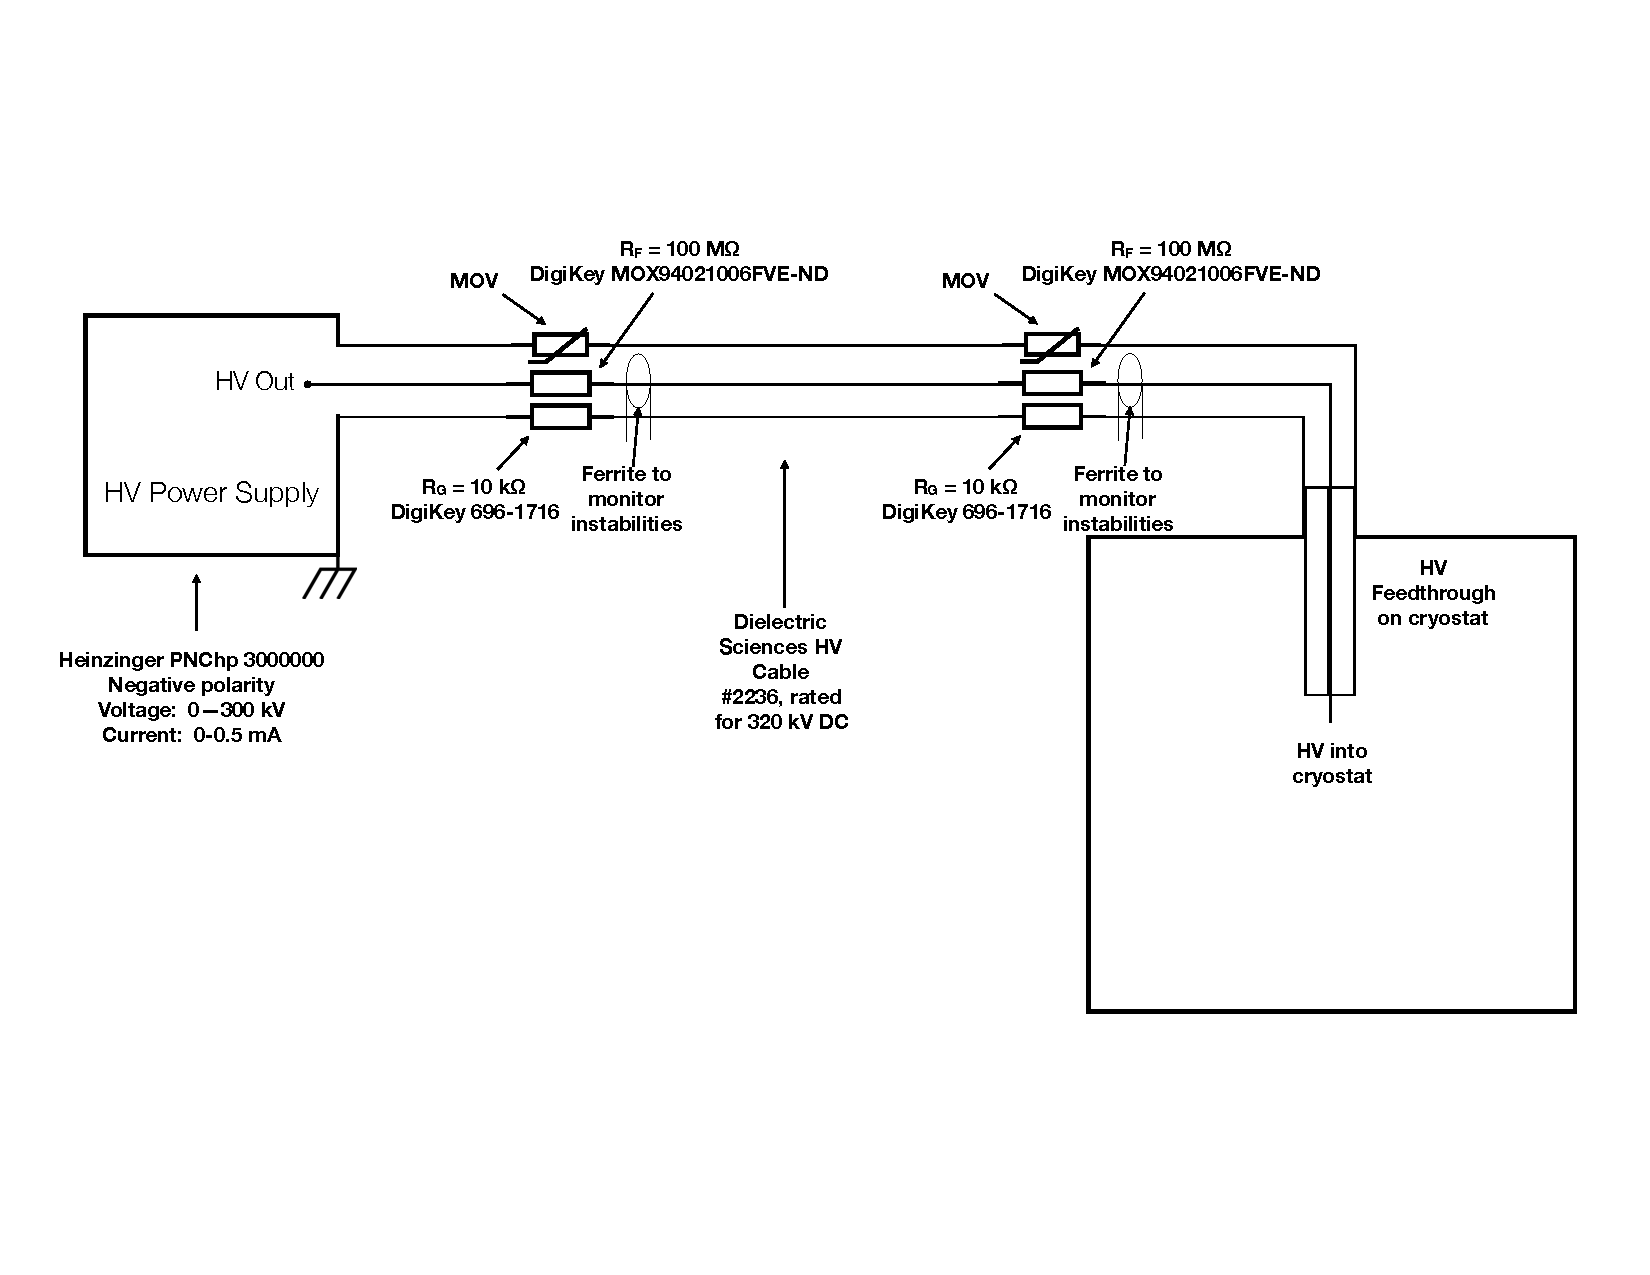
\includegraphics[width=0.6\textwidth]{ps_filter_ft_schematic}
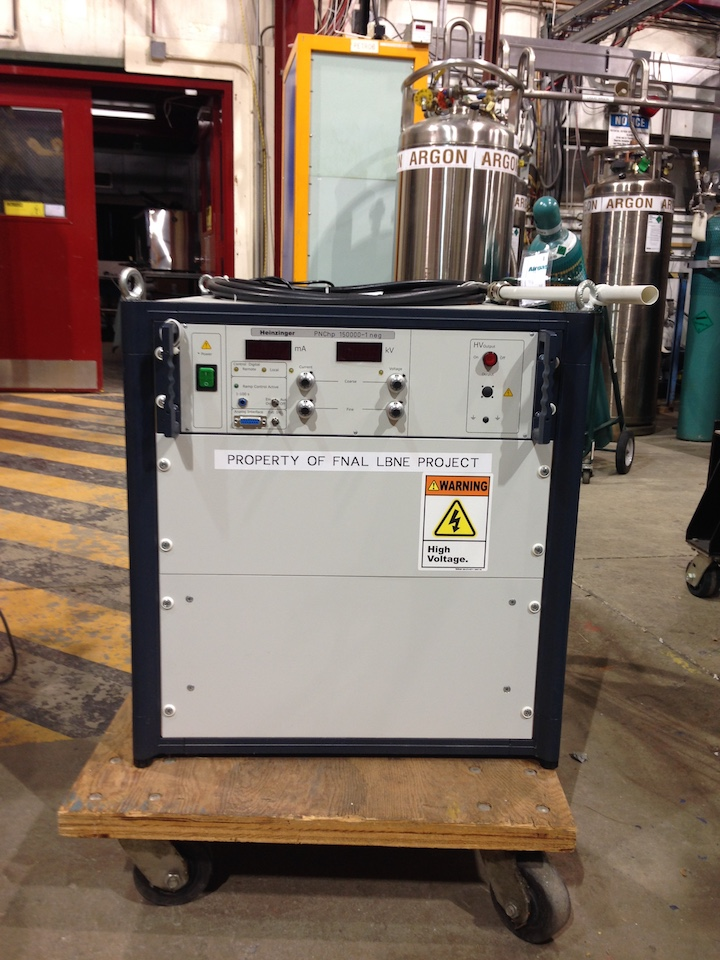
\includegraphics[width=0.3\textwidth]{heinzy}
\end{dunefigure}
The filter resistors will be placed in between the power supply and the feedthrough.  Along with the cables, they reduce the discharge impact by partitioning the stored energy in the system.  The resistor-cable assembly also serves as a low-pass filter reducing the $\sim$\SI{30}{kHz} voltage ripple on the output of the power supply.

The requirement of low electronics noise will set the upper limit of residual voltage ripple on the cathode, likely to be $\sim$\SI{0.5}{mV}.  Typically, commercial supplies can specify the ripple to be less than or equal to $0.001\%V_{nom} \pm 50$ mV.  Assuming cable lengths of \SI{30}{m} and \SI{3}{m} between the filters, and between the filter and feedthrough, the noise reduction can be attained with resistances as low as a few M$\Omega$. 

The current plan for the filters is a cylindrical design.  Here, a high voltage resistor will be electrically connected on each end to a cable receptacle.  The resistor should be selected to withstand a large over-power condition.  Radially out from the resistor is an insulator.  In other designs, this has been transformer oil or Ultra-high-molecular weight Polyethelene (UHMW-PE).  The outer case of the filter is a grounded stainless-steel shell.

The high voltage feedthrough will be based on the successful ICARUS design, which has been adapted for ProtoDUNE.  The voltage is transmitted by a stainless steel center conductor.  On the warm side of the cryostat, this conductor mates with a cable end.  Inside the cryostat, the end of the center conductor has a spring-loaded tip that will contact a receptacle cup mounted on the cathode delivering high voltage to the field cage.  The center conductor of the feedthrough is surrounded by UHMW PE.  The upper bound of operating voltage on a feedthrough is, to first order, set by the maximum electric field on the feedthrough.  This electric field is reduced by increasing the insulator radius.  For the target voltage, the feedthrough will use a UHMW PE cylinder of roughly 15 cm diameter.  In the gas space and into at least 15 cm of the liquid, the insulator will be surrounded by a tight fitting stainless steel ground tube.  The ground tube will have a 25 cm Conflat flange welded on for attachment to the cryostat.

There will be multiple devices used to monitor the high voltage.  Outside of the cryostat, the power supply and cable-mounted toroids will be used.  The Power Supply units typically have sensitivities down to 10's of nA in current read-back capability.  The units are able to sample the current and voltage every \SI{300}{ms}.  The cable-mounted toroids are sensitive to fast changes in current and can be monitored when desired.  The polarity of the signal also points to whether the current-drawing feature is upstream or downstream of the toroid.

Inside the cryostat, pick-off points near the anode will monitor the current going down each resistor chain.  Additionally, the voltage of the Ground Planes above and below each drift region can be equipped to diagnose problems via a diode-to-cryostat ground.


\subsection{Cathode Plane Assembly (CPA)}

The CPA provides a constant potential surface at -180 kV for the DUNE SP TPC.  It receives its high voltage from the HV Feedthrough which makes contact with the HV Bus mounted on the CPA frame through an attached donut assembly. Figure~\ref{fig:donut_cpa} shows the connection of the HV input donut to the HV Bus on the CPA frame. 

\begin{dunefigure}[HV input donut connection to CPA]{fig:donut_cpa}{HV input donut connection to CPA.}
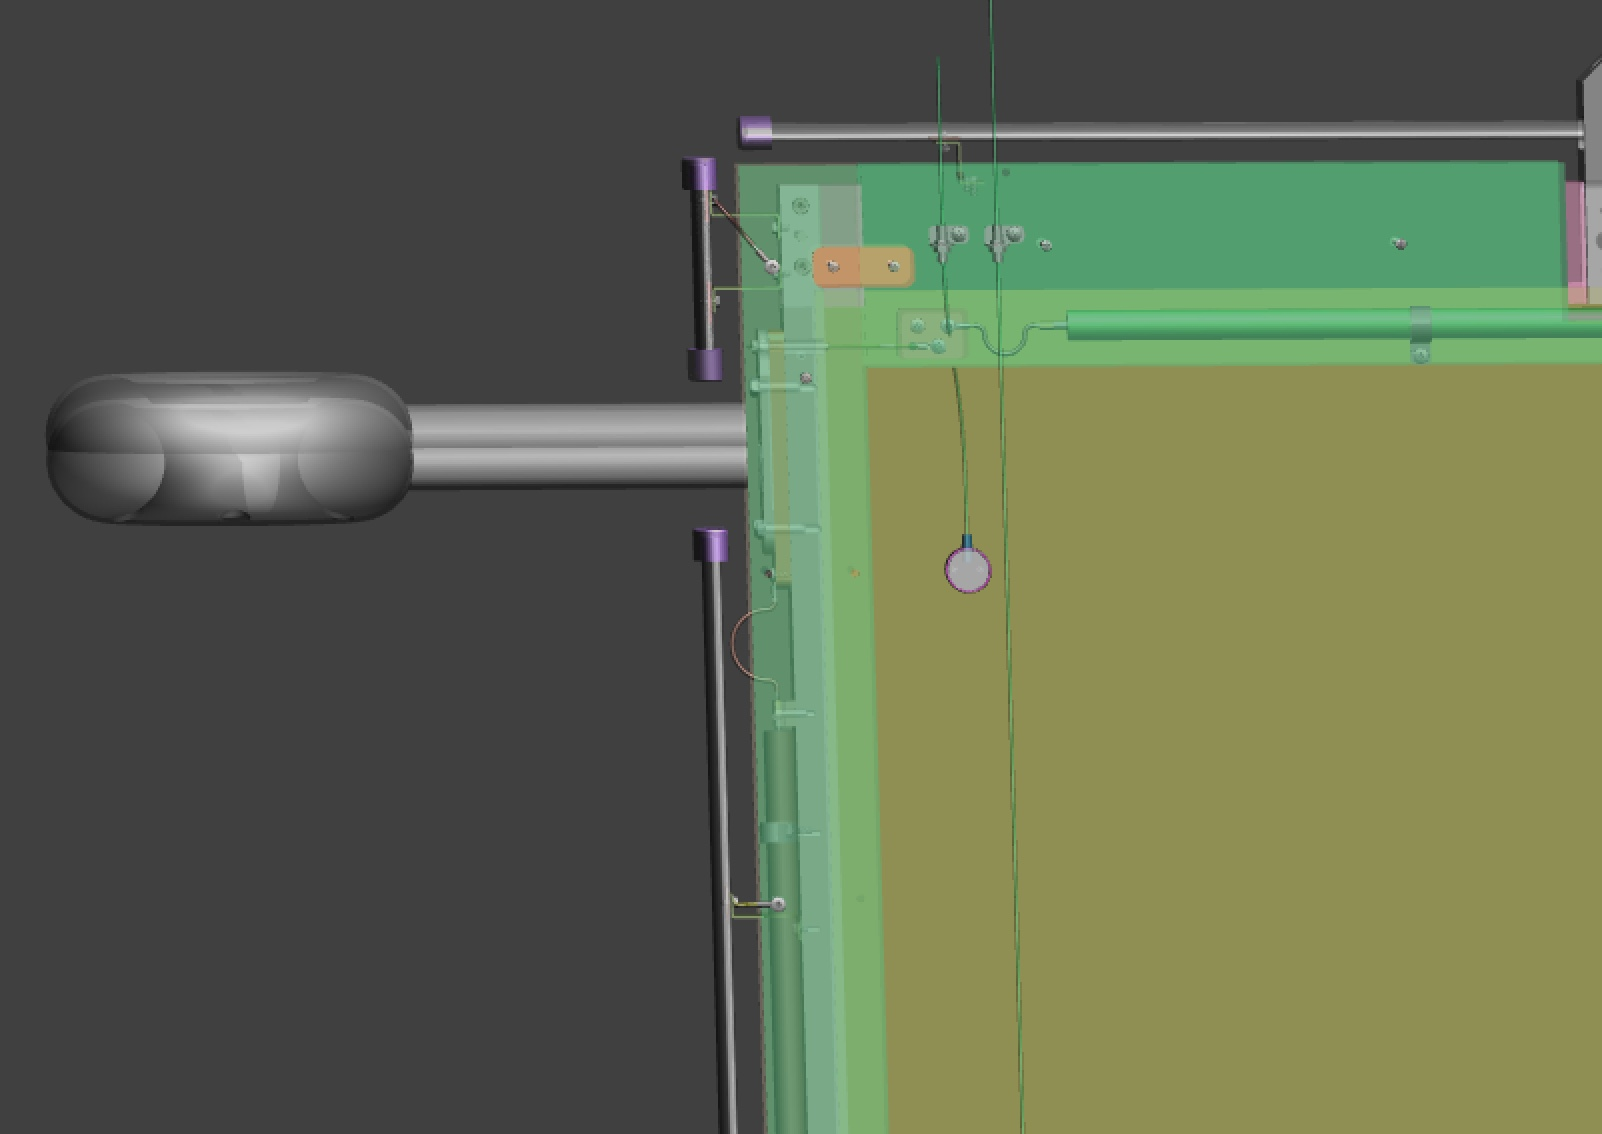
\includegraphics[width=0.6\textwidth]{donut_cpa} %{ was Latest3D}
\end{dunefigure}

The CPA also provides HV to the first profile on the Top and Bottom Field Cage (FC) elements and to the EndWall-FCs as well. More details of the electrical connections are found in Section ~\ref{sec:fdsp-hv-design-interconnect}.

The constant potential surfaces are resistive panels (CPA-RP's) comprised of a thin layer of carbon-impregnated kapton laminated to both sides of a 3 mm thick FR4 sheet of 1.2 m X 2 m size.  The surface resistivity of the CPA-RP's is required to be in the range of 1-10 MOhms/square in order to provide for slow reduction of accumulated charge in the event of a discharge.  Other HV components of the CPA include field shaping strips (FSS's) mounted to the CPA frames, edge aluminum profiles to act as the first elements of the field cage, and cable segments forming the HV Bus. Careful inspection of these items during the assembly process ensures that no sharp points or edges are present. Figure~\ref{fig:cpa_panel-complete} shows a completed CPA Panel on the production table ready for lifting into vertical position for mounting on its trolley.

\begin{dunefigure}[Completed ProtoDUNE CPA Panel on production table]{fig:cpa_panel-complete}{Completed ProtoDUNE CPA Panel on production table.}
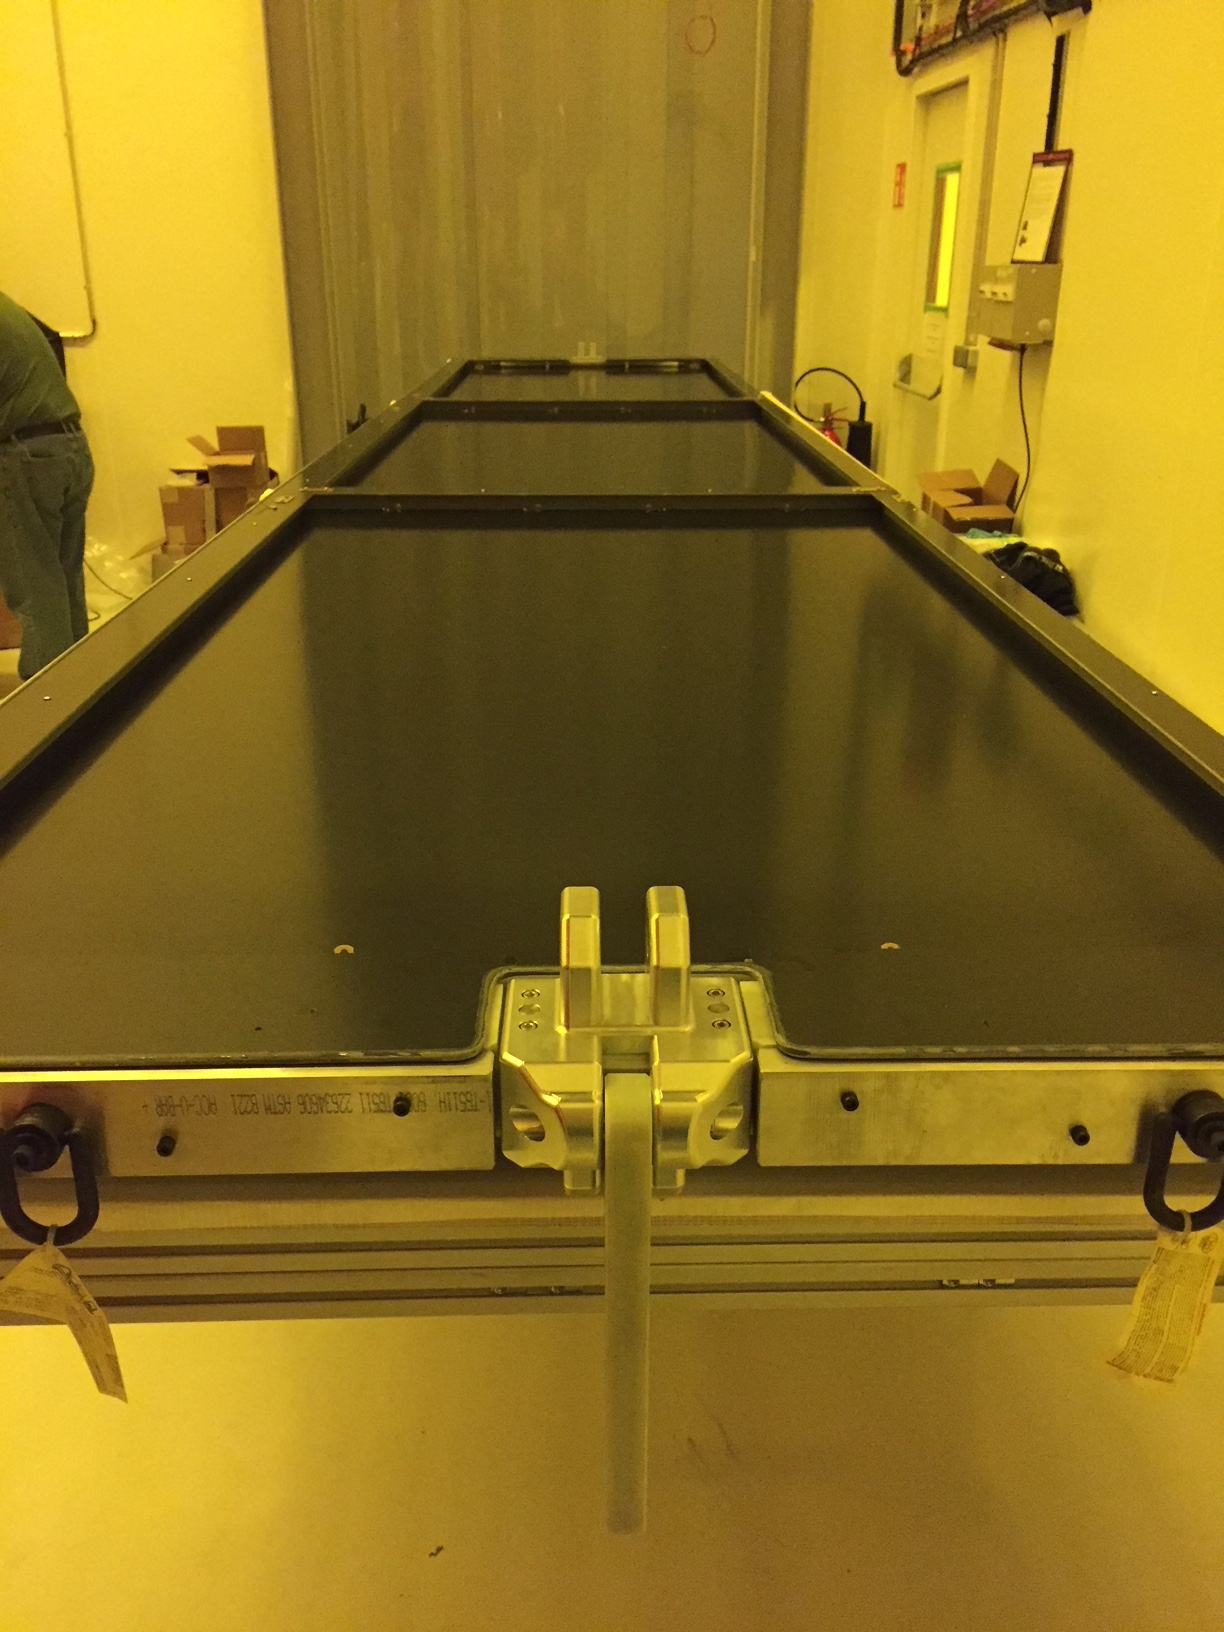
\includegraphics[width=0.5\textwidth]{cpa_panel-complete}
\end{dunefigure}

The CPA frames are required to support, in addition to the HV components, Top and Bottom FC units attached to both sides of the CPA panel. The arrangement and deployment of these components will be the same as in ProtoDUNE.  

\subsection{Field Cages}

\subsubsection{General Considerations}

A uniform electric field is required to drift ionization electrons towards the APAs. Field cages consisting of field shaping electrodes form a band surrounding the top, bottom, and ends of the active drift volume. The electrodes are biased at different potentials to establish a uniform field inside the LAr volume.
The DUNE SP far detector will use extruded aluminum profiles as a cost effective way to establish the equipotential surfaces. 

The shape of the electrodes is critical as it determines the strength of the electric field between a given profile and its neighboring profiles as well as
other surrounding parts, including the APA, which is electrically at ground level. Electric fields need to be well below 30kV/cm 
to enable safe TPC operation.

The commercially available profiles used for ProtoDUNE, and forming the DUNE design, are estimated to lead to E fields of up to 12~kV/cm under the assumption of DUNE field cage configuration 
and operating voltage. Figure \ref{fig:profile-e-field} illustrates results from a E field calculation.

\begin{dunefigure}
[Electric field map (color) and equipotential contours of an array of roll formed profiles biased up to -180kV and a ground clearance of 20cm]{fig:profile-e-field}
{Electric field map (color) and equipotential contours of an array of roll formed profiles biased up to -180kV and a ground clearance of 20cm(Credit: CAD model)} 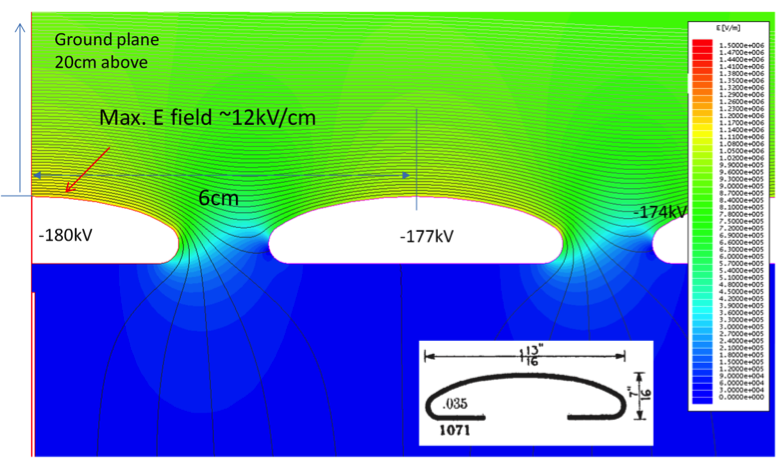
\includegraphics[width=0.8\textwidth]{profile-e-field.png}
\end{dunefigure}

The profiles ends are equipped with UHMW polyethylene caps to reduce the risk of arc formation.  These caps are designed to have sufficient wall thickness (6mm) to withstand the full voltage across their walls.

The Aluminum profiles are attached to fiber-reinforced plastic (FRP) pultruded structural elements, including I-beams and box beams.  
Pultruded FRP material is non-conductive and strong enough to withstand the loads of field cage in the temperature range of -150C and 23C.
%FRP has all of the reinforcing fibers running along the main axis of the section being used.  
The FRP material will meet the International Building Code classification for flame spread and smoke development of a Class A, as characterized by ASTM E84.  


As discussed in the Introduction, the field cage modules have two types: the top/bottom (T/B), and the end wall both of which are described below. 
A resistive divider chain interconnects all the Aluminum profiles to provide a linear voltage gradient between the cathode and anode planes.  The T/B modules are nominally 2.3m wide by 3.6m long. A ground plane in the form of tiled perforated stainless steel sheet panels is mounted on the outside surface of the T/B field cage module with a 20cm clearance. The T/B modules are supported by the CPAs and APAs. The end wall modules are 1.5m tall by 3.6m long. They are stacked 8 units high (12m), and are supported by the installation rails above the APAs and CPAs.



\subsubsection{Top and Bottom field cages (FC)}

The top and bottom (T/B) field cage modules are 3.52~m long, which is set by the length of the two 15 cm (6-inch) FRP I-beams that form the primary support structure of the modules. The I-beams are connected to each other by three  7.5 cm (3-inch) FRP cross beams. The connections between the longitudinal and cross I-beams are made with L-shaped FRP braces that are attached to the I-beams with FRP spacer tubes, and secured with FRP threaded rods, FRP hex-head nuts, and custom-machined FR4 washer plates.

The modules are 2.3~m wide, which corresponds to the length of the aluminum profiles, including the UHMW polyethylene end caps. Profiles are secured to the FRP frame using custom-machined double-holed slip nuts that are slid into the profiles such that they straddle the webbing of the 15 cm I-beams, and are held in place with screws that penetrate the I-beam flanges. The profile offset with respect to the FRP frame is different for modules closest to the endwalls, and modules in the center of the active volume.

Each T/B module holds 5 ground planes, which are connected to the outside (i.e. non-drift side) of the module. The ground planes are positioned $\sim$20.5~cm above the profiles, and are pushed to the CPA side of the module, leaving the last 14 profiles (88~cm) on the APA side of the module exposed. Between the ground planes and the 15 cm I-beams are standoffs made of short sections of 10 cm (4 inch)  FRP I-beams, which are connected with FRP threaded rods and slip nuts. The electrical connection between the ground planes is made with copper strips.

The connections between the T/B modules and the CPAs are made with aluminum hinges, 2.5 cm (1 inch) in thickness, that allow the modules to be folded in to the CPA during installation. The hinges are electrically connected to the second profile from the CPA. The connections to the APAs are made with stainless steel latches that are engaged once the T/B modules are unfolded and fully extended toward the APA.

The voltage drop between adjacent profiles is facilitated by voltage divider boards that are screwed into the drift volume side of the profiles. A custom machined nut plate is used that can be inserted into the open slot of each profile and twisted 90$^\circ$ to lock into position. Two additional boards to connect the modules to the CPAs were screwed into the last profile on the CPA side of the module. This system is also described in section ~\ref{sec:fdsp-hv-design-interconnect}. A fully assembled module is shown in Figure~\ref{fig:tbfc1-2}.

\begin{dunefigure}[Top/Bottom Field Cage Modules]{fig:tbfc1-2}{The fully assembled modules with ground planes is shown (left), as well as a close up of CPA end as viewed from the bottom (drift) side of the module.}
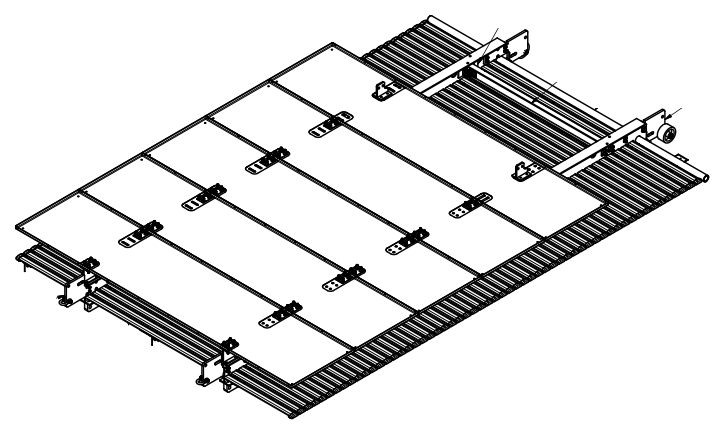
\includegraphics[width=0.65\textwidth]{tbfc1}
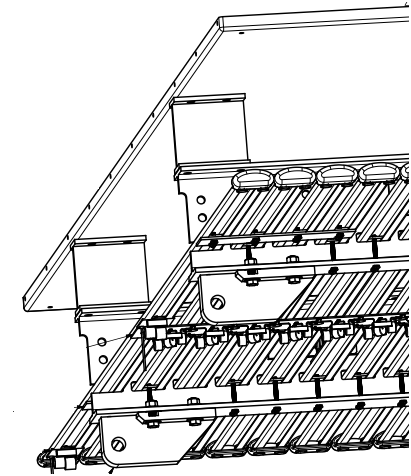
\includegraphics[width=0.33\textwidth]{tbfc2}
\end{dunefigure}


\subsubsection{ Endwall field cages (EW-FC}

The End Wall Field Cage (EWFC) for each of the 4 drift volumes consists of two Endwalls (EW), one on each side of the drift volume. Each Endwall is in turn composed of 8 Endwall Modules (EW-Modules). 

There are two different types of EW-Modules, each of which comes in a "regular" and in a "mirrored" configuration to account for 
mounting constraints and to match the detector geometry. Figure \ref{fig:fc_endwall_panels} illustrates the layout for the topmost 
and the baseline panels, respectively.

\begin{dunefigure}[Endwall Field Cage Panels]{fig:fc_endwall_panels}{Left: Uppermost panel of the Endwall Field Cage. Right: Baseline Endwall Field Cage Panel.}
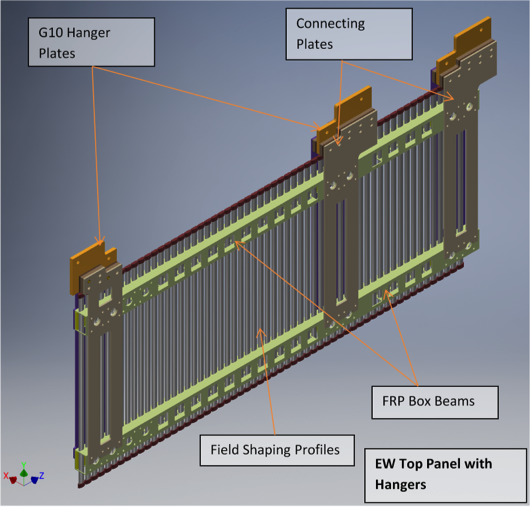
\includegraphics[width=0.48\textwidth]
{fc_endwall_top_panel}
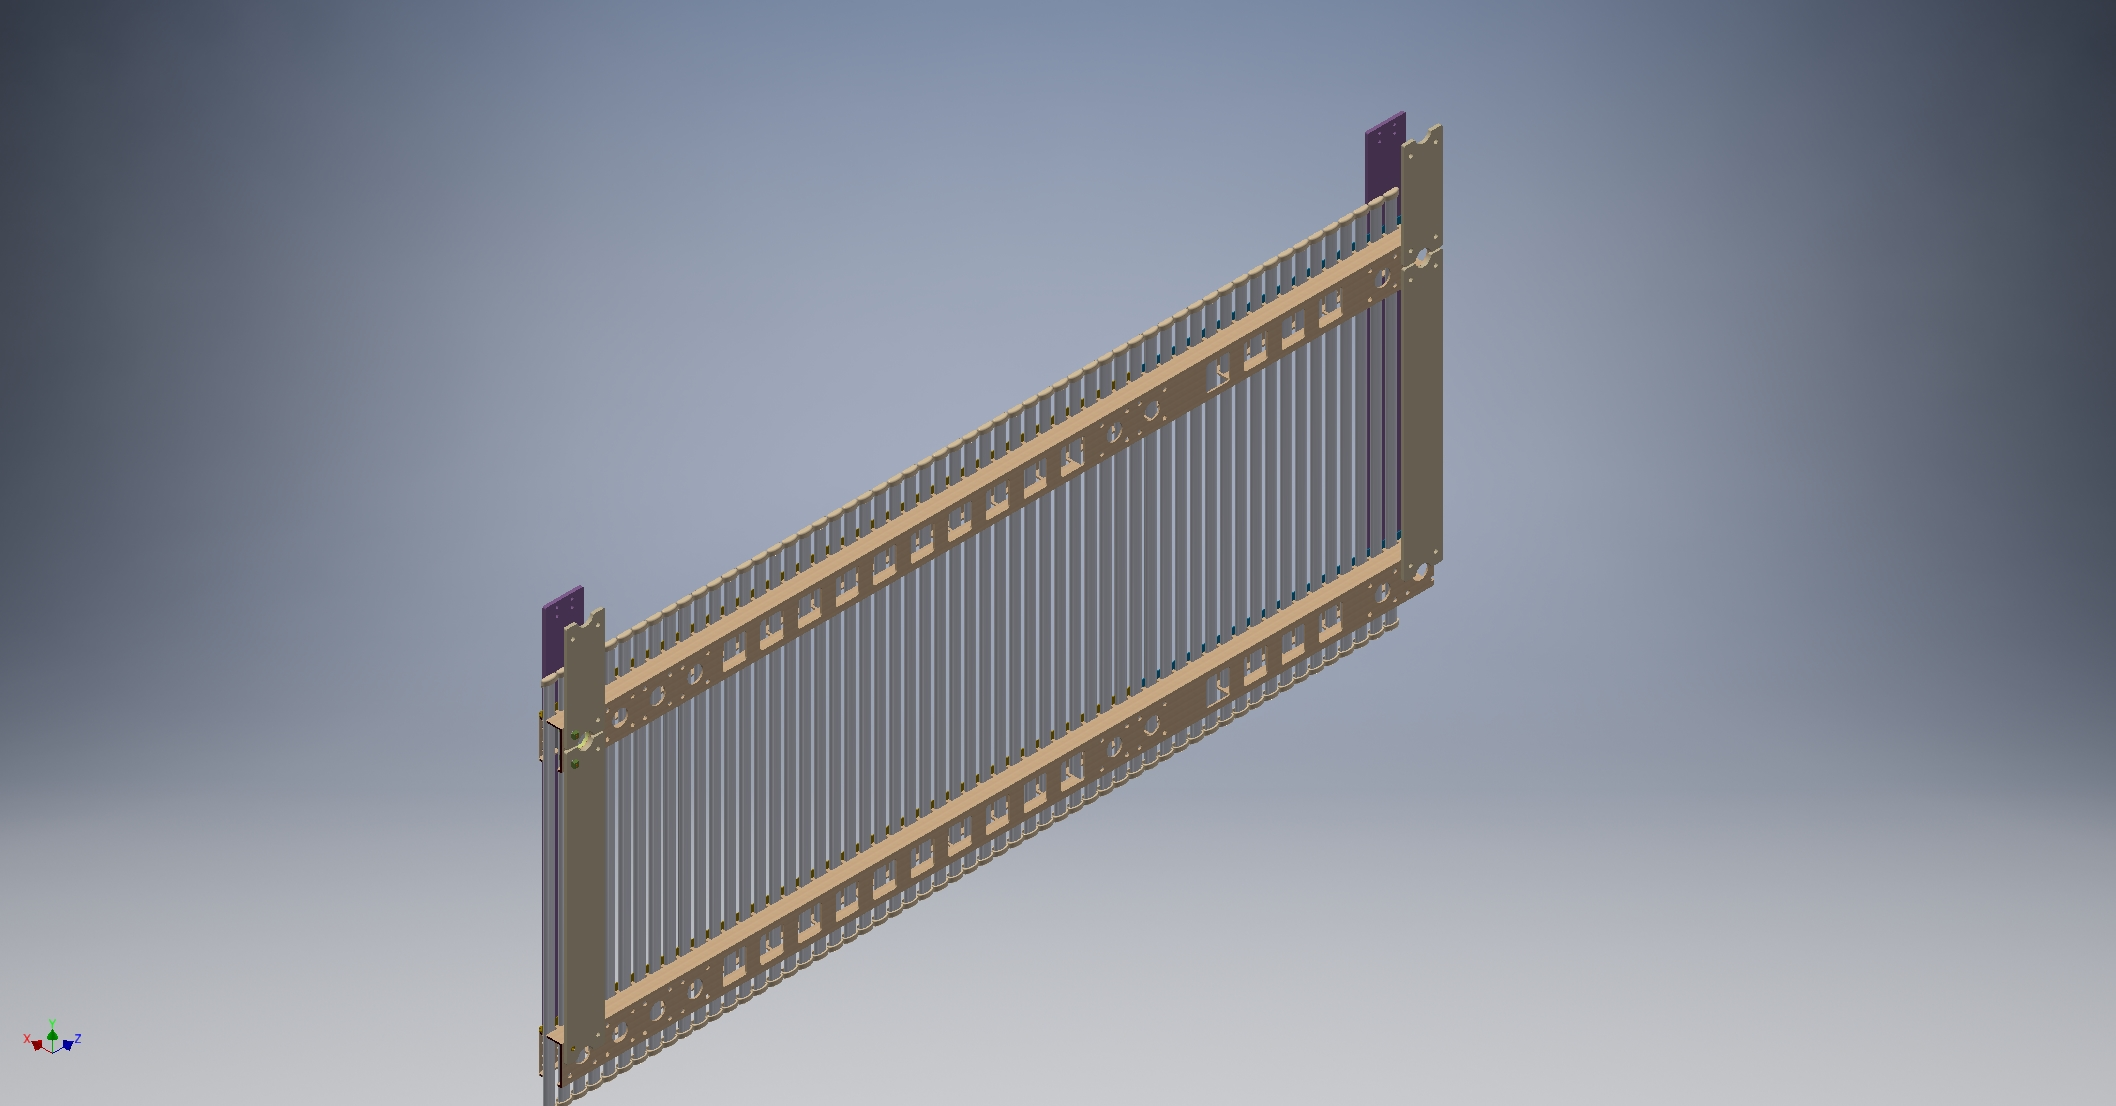
\includegraphics[width=0.48\textwidth]
{fc_endwall_panel}
\end{dunefigure}

Each EW-Module is constructed of two FRP box beams which are 3.6 m long. The box beam design also incorporates cutouts on the outside face to minimize charge build up. Box beams are connected using 1.3 cm (1/2 inch) thick FRP plates. The plates are connected to the box beams using a shear pin and bolt arrangement. The inside plates facing the active volume are connected using special stainless steel slip nuts and stainless steel bolts. The field shaping profiles are connected to the top box beam using stainless steel slip nuts, an FRP angle, and two screws each. The profiles are connected to the bottom box beam with a slip nut that is held in place by friction.

%\begin{center}
%   \parbox[t]{0.47\textwidth}{
 %  \resizebox{0.47\textwidth}{!}{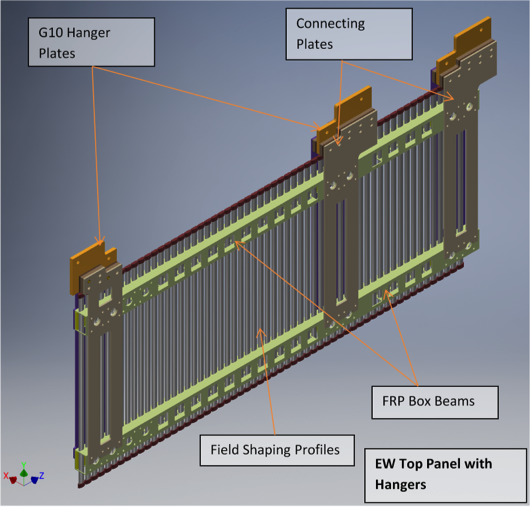
\includegraphics[width=0.48\textwidth]{FCendwall_top-panel.png}}
%\caption{\label{fig:FCendwall_top} Uppermost panel of the field cage endwall. {\color{red} NOTE: need to replace figure with updated version for DUNE, e.g. without middle FRP cross member.}}}
%\makebox[0.025\textwidth]{}
 %  \parbox[t]{0.48\textwidth}{
 %  \resizebox{.48\textwidth}{!}{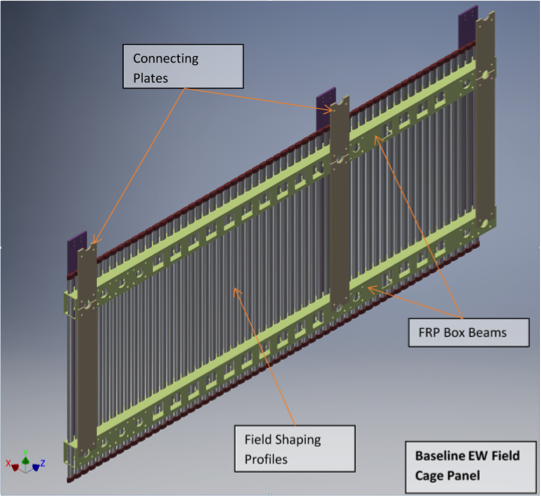
\includegraphics[width=0.48\textwidth]{FCendwall_panel.png}}
%\caption{\label{fig:FCendwall_panel} Baseline field cage panel. {\color{red}NOTE: need to replace figure with updated version for DUNE, e.g. without middle FRP cross member.}}}
%\end{center}


\subsection{Electrical Interconnections} % (Glenn)
\label{sec:fdsp-hv-design-interconnect}

\begin{dunefigure}[HV Interconnection Topology]{fig:fdsp-hv-design-interconnect-concept}
  {High-level topology of the HV interconnections}
  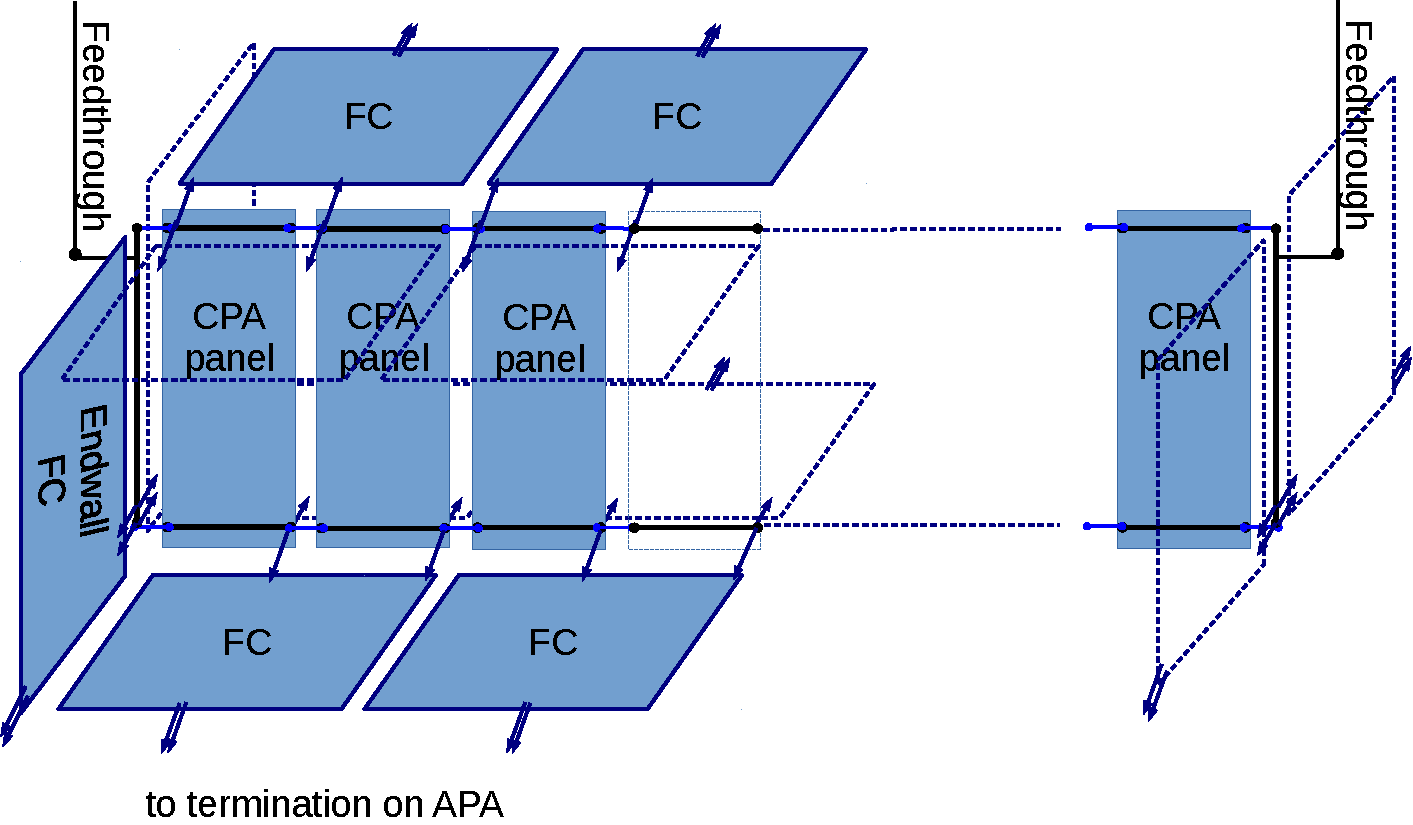
\includegraphics[width=0.7\textwidth]{fdsp-hv-interconnection-topology}
\end{dunefigure}

Electrical interconnections are needed among the HV delivery system, CPA planes, field cage modules, and termination
boards on the APA modules, as well as between resistive dividers and
the field-forming elements on the CPA's and field cages.  Redundancy is
needed to avoid single points of failure.  Some connections must be
insulated in order to avoid creating a discharge path that might
circumvent the discharge mitigation provided by the resistive CPA
surface and field cage partitioning.  Certain connections must be
flexible in order to allow for field cage deployment, thermal
contraction, and motion between separately supported CPA's.  Figure
\ref{fig:fdsp-hv-design-interconnect-concept} shows a high level
overview of the interconnections between the HV, CPA, and FC modules.


%% connections between major elements (HV, CPA, FC, APA)
High voltage feedthroughs connect to cups mounted on the CPA frame
%\cite the HV delivery section
which attach to a HV bus running through the CPA's.  HV bus connections
between CPA panels are made by flexible wires through holes in the
CPA frame. The HV bus is a loop in order to mitigate risk of a single
point failure; feedthroughs at each end of each CPA plane mitigate
risk of a double-break failure.  Voltage dividers on each CPA panel
bias the field shaping strips and the resistive dividers on the top
and bottom field cages.  CPA-to-field cage connections are made using
flexible wire to accommodate field cage deployment.  To further
increase redundancy, two CPA panels connect to each top or bottom
field cage, and two connections are also made to each endwall.  Field
cage resistor divider boards attach directly to the interior side of
the FC profiles with screws.  A redundant pair of flexible wires
connects a circuit board on the last profile of each field cage to a
bias-and-monitoring board mounted on the corresponding APA.

%% connections within CPA
Short sections of flexible wire at the ends of each HV bus segment
attach to screws in brass tabs on the CPA resistive panels (CPA-RP's).
%\cite CPA design subsection
Vertical HV bus segments on the outer ends of each CPA-Plane connect
the top and bottom HV buses to complete the loop.  Solid wire is used
to connect resistive panels within a CPA-Panel.

%% FC connections
Each field cage is as electrically independent as possible in order to
mitigate discharge.  However, only the bottom module of each endwall
can make connections to the HV bus and APA, so each endwall module
will be connected to its upper neighbor at its first and last profiles
using metal strips.

%% Regarding wire terminals and screws
All flexible wires have ring or spade terminals and are secured by
screws in brass tabs.  Spring washers are used with every electrical
screw connection in order to maintain good electrical contact with
motion and changes of temperature.

Table \ref{tab:sp-hv-interconnects} summarizes the interconnections
required.

\begin{dunetable}
[HV System Interconnections]
{p{0.35\linewidth}p{0.62\linewidth}}
{tab:sp-hv-interconnects}
{HV System Interconnections}   
 Connection & Method \\ \toprowrule
 HV cup to HV bus & wire to screw in HV cup mount on CPA frame \\
 HV bus between CPA-Panels & wire between screws in brass tabs \\
 HV bus to FSS & wire to circuit board mounted on FSS \\
 FSS to FC (top/bottom) & wire to circuit board on first FC profile, two per FC module \\
 HV bus to Endwall FC & wire to circuit board mounted on first FC profile, two per Endwall \\
 FC divider circuit boards & directly attached to profiles using screws \\
 FC to bias/monitoring termination & redundant wires from board mounted on last FC profile \\
 HV bus to CPA-Panels & brass tab on CPA resistive panel \\
 CPA-RP interconnections & solid wire between screws in brass tabs \\
 Endwall FC module interconnections & metal strips, first and last profiles only
 \\
\end{dunetable}



%%%%%%%%%%%%%%%%%%%%%%%%%%%%%%%%%%%
%\subsection{Quality Assurance}
%\label{sec:fdsp-hv-qa}


%%%%%%%%%%%%%%%%%%%%%%%%%%%%%%%%%%%%%%%%%%%%%%%%%%%%%%%%%%%%%%%%%%%%
\section{Production and Assembly}
\label{sec:fdsp-hv-prod-assy}

%%%%%%%%%%%%%%%%%%%%%%%%%%%%%%%%%%
\subsection{Power Supplies and Feedthroughs}
\label{sec:fdsp-hv-supplies-feedthroughs}

Additional power supplies will be commercially procured, for example through Heinzinger. The high voltage cable is commercially available.

The power supply will be tested extensively along with the controls and monitoring software.  Features to be included in the software are:
\begin{itemize}
\item The ability to ramp, or change the voltage.  The rate and an ability to pause the ramp shall be included.
\item An input for a user-defined current limit.  This parameter is the current value at which the supply reduces the voltage output to stay below the current limit.  The current limiting is done in hardware.
\item An input for a trip threshold.  At this current reading, the program would reduce the voltage output through software.  In previous experiments, the trip function in software would set the output to \SI{0}{kV}.
\end{itemize}
\noindent Additionally, the software should record the current and voltage read back values with a user-defined frequency, and also any irregular current or voltage events.

The high voltage feedthroughs, filters, and splitter are custom devices.  One feedthrough option is to use the ProtoDUNE-SP design and similar procurement.  High voltage splitters are already on hand if they are desired.

%%%%%%%%%%%%%%%%%%%%%%%%%%%%%%%%%%
\subsection{CPA}
\label{sec:fdsp-hv-prod-cpa}

The component parts of the CPA assembly will be produced by commercial vendors for the following items:
\begin{itemize}
\item Manufactured FR4 RP frames packed into 3 CPA-Unit kits making up a CPA Panel
\item Carbon-impregnated Kapton coated resistive panels (RPs) and Field Shaping Strips (FSSs)
\item HV cable segments and wire jumpers making up the CPA HV Bus and RP interconnects
\item Machined Brass tabs for connecting RPs, HV Bus, and FSSs
\item Top, Bottom, and exterior edge profiles
\end{itemize}
The above items will be packaged into CPA-Panel kits by the vendors and will be sent to the assembly factories.  The basic construction unit for an assembly factory will be a pair of CPA-Panels so that shipment to SURF from an assembly factory will consist of two CPA-Panels that are paired on site to form a CPA-Plane.

The most basic element of the CPA is a RP mounted in a machined slot in the top, bottom and sides of FR4 frames.  There are three different types of these CPA-RP elements - an Upper which has as its top frame the CPA mounting bracket and Top FC hinge, a Middle, and a Lower which has as its bottom frame a Bottom FC hinge.  Two such CPA-RP elements are bolted together and pinned to form a shipment CPA-Unit of size 1.2 m X 4 m.  These CPA-Units are assembled horizontally on a smooth, flat table to meet the dimensional requirements of CPA construction.  In addition to the frames and RPs, FSSs are mounted on the exposed sides of the FR4 frames, aluminum profiles are attached to the top and bottom of the Upper and Lower elements, and cables are attached to the RPs to form segments of the HV Bus.  The shipment CPA-Unit comes in 3 varieties in order to make a full 12 m tall CPA Panel.  These are : 1) an Upper CPA-RP element attached to a Middle element, 2) two Middle elements connected, and 3) a Middle element attached to a Lower element.  The CPA-Unit order in the shipping crate from bottom to top is Middle/Lower, Middle/Middle, Upper/Middle.  For the 10 kt DUNE SP TPC, there are 100 Upper elements, 100 Lower elements and 400 Middle elements which make up the 100 CPA Panels of the TPC.
A comparison of a 6 m ProtoDUNE SP CPA Panel and a 12 m DUNE SP Panel is shown at Ash River in Figure~\ref{fig:12m-cpa}.

\begin{dunefigure}[CPAs at Ash River]{fig:12m-cpa}{A 6 m ProtoDUNE CPA Panel and a 12 m DUNE CPA Panel mockup at Ash River.}
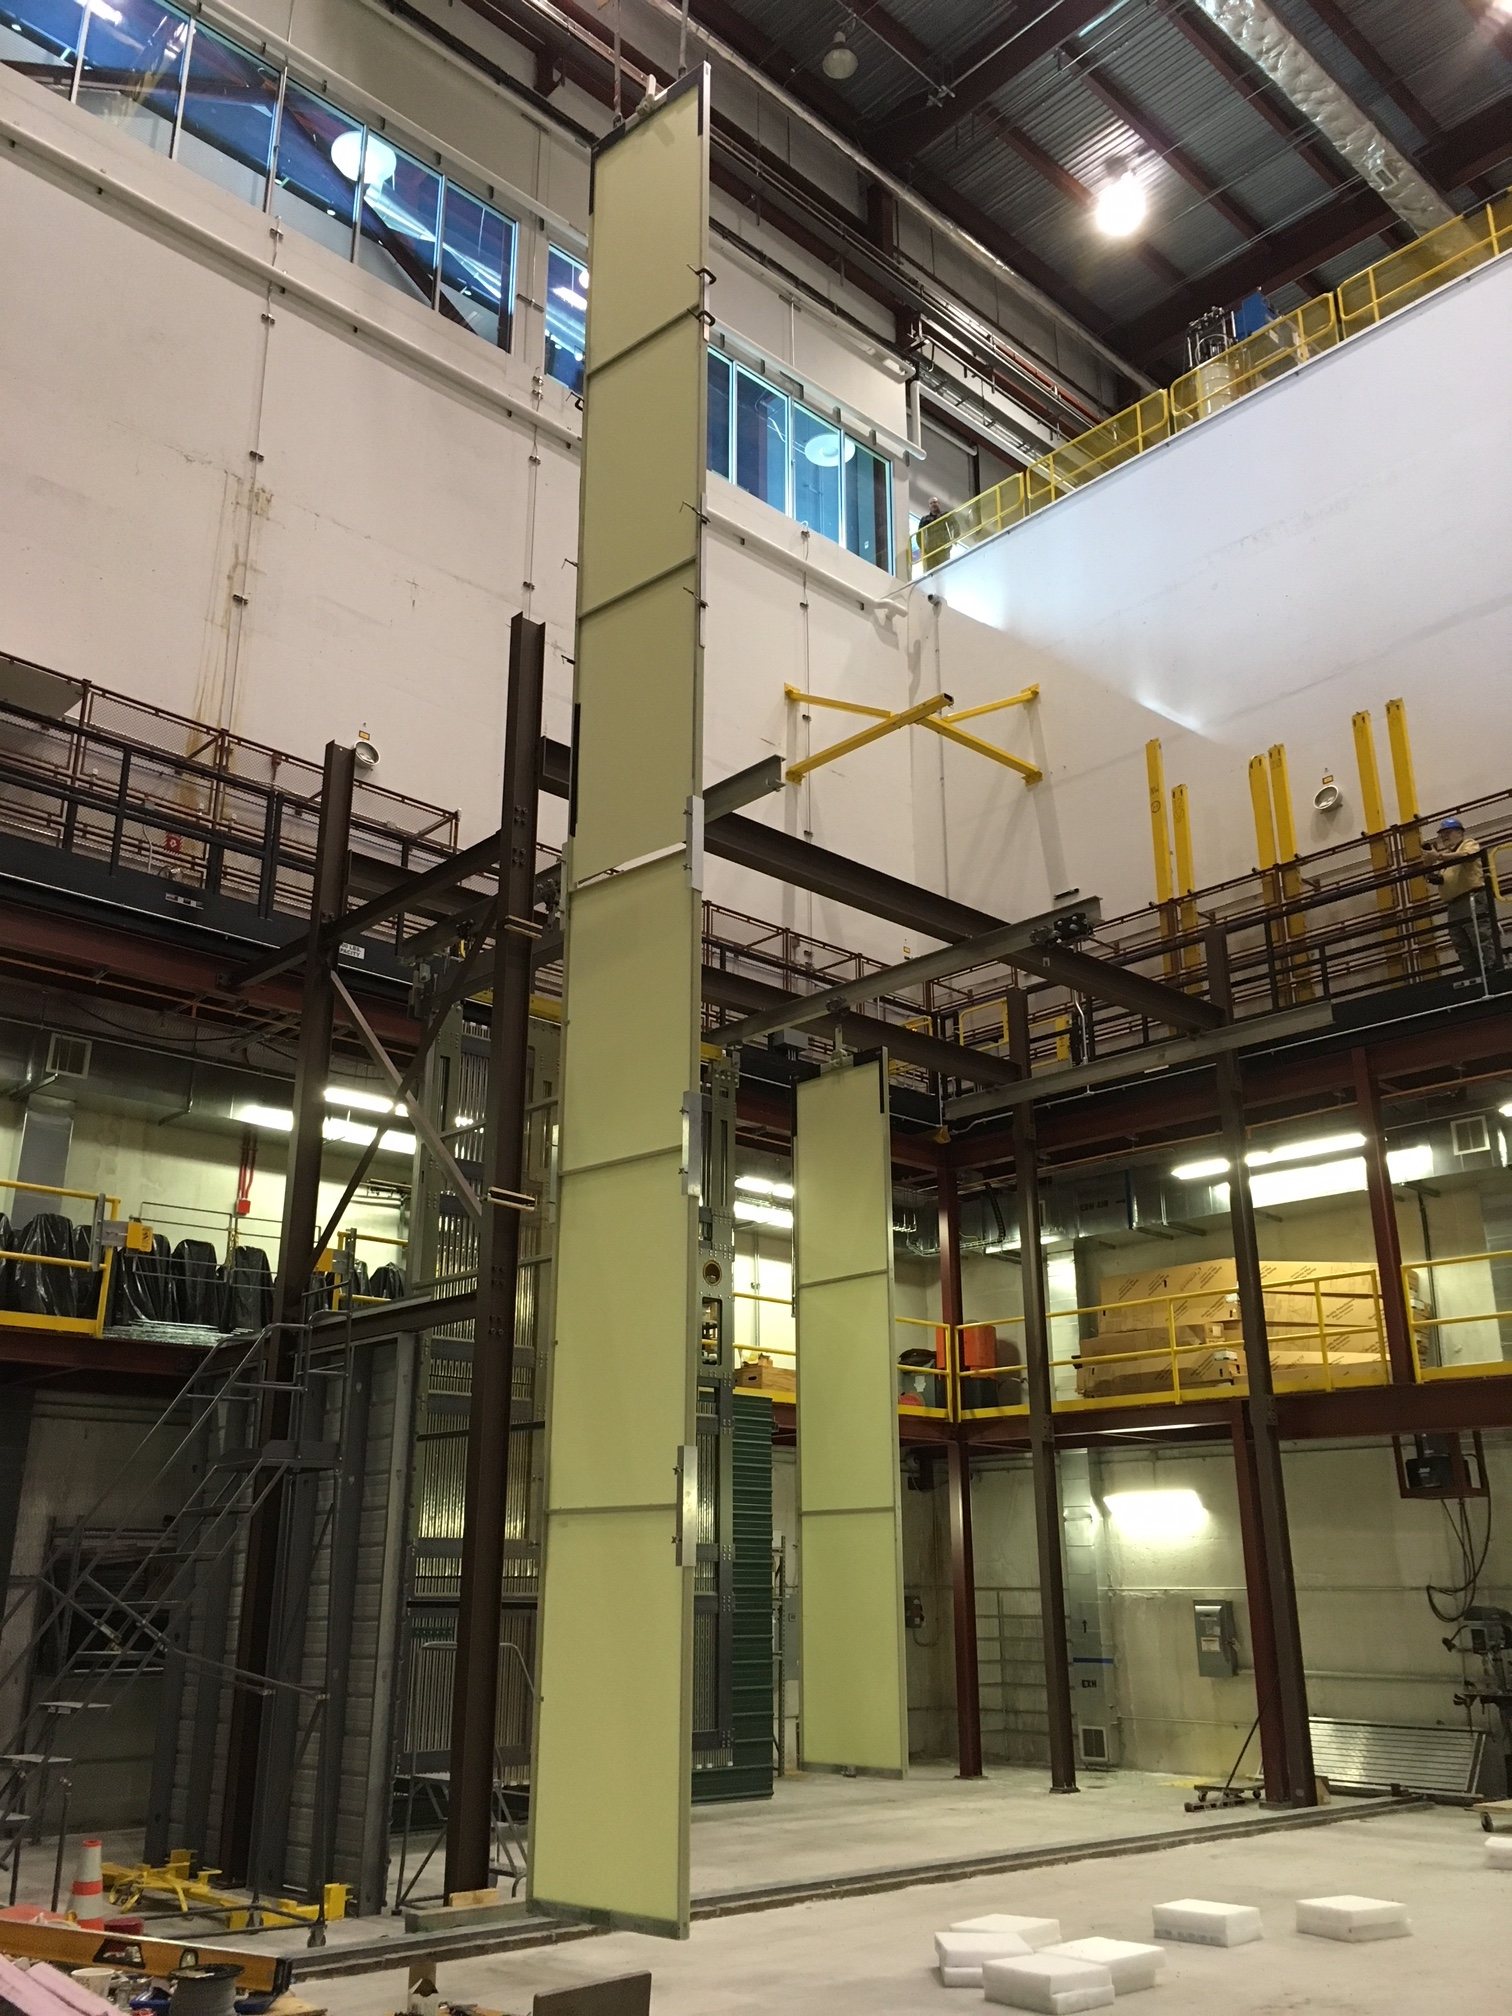
\includegraphics[width=0.35\textwidth]{12m-cpa}
\end{dunefigure}

\subsection{Field Cages}
\label{sec:fdsp-hv-prod-fc}

% Include profile procurement & QC here


\subsubsection{Top and Bottom Field Cages (FC)}

%Discussion of parts procurement, assembly, and testing.
The FRP and FR4 components of the top and bottom (T/B) FC's will be commercially produced by firms which specialize in the machining of fiberglass components for electrical applications, as was successfully done for ProtoDUNE. All parts are machined in the absence of water and cleaned with a lacquer thinner. Machined edges, other than small circular holes, will be coated with translucent epoxy. The stainless steel and aluminum components will be produced in local university and commercial machine shops. The voltage divider boards will be provided by Louisiana State University, and the boards used to make the FC/CPA connection will be provided by Kansas State University.

The FRP frame assembly primarily consists of fastening together FRP I-beams with FRP threaded rods and hex nuts, which are secured with a limited and specified torque, to avoid damage to the threads. A detailed view of one of these connections is shown in Figure~\ref{fig:tbfc3}.

\begin{dunefigure}[Top/Bottom Field Cage Module Frame Assembly]{fig:tbfc3}{The components (left) and assembled view (middle and right) for the FRP frame connections in Top/Bottom Field Cage modules are shown.}
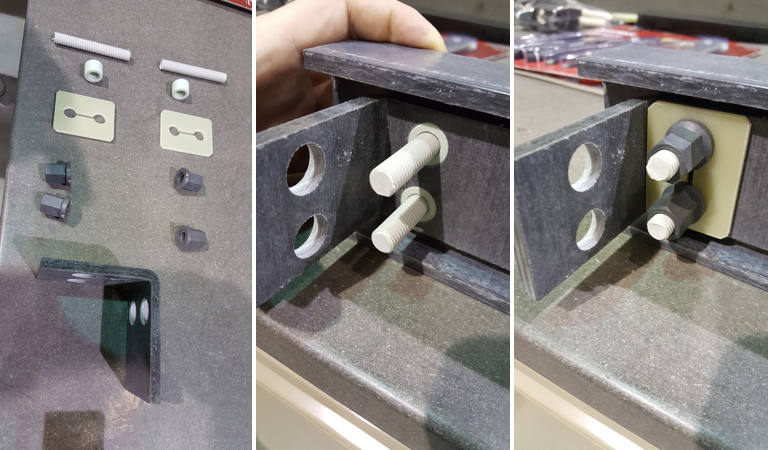
\includegraphics[width=0.85\textwidth]{tbfc3}
\end{dunefigure}

Prior to sliding each profile into the FRP frame, the holes should be covered with kapton tape to avoid damage to the profile coating. An end cap is attached to each profile using plastic rivets, and then the profiles are aligned against an aligment fixture running the length of the FC. After securing each profile to the frame, the tension in the mounting screws is adjusted to remove any angular deflection in the extended portion of the profile.

The ground planes are attached to the 10 cm stand-off I-beam sections with threaded rods and a machined plate. The copper strips are connected to adjacent modules at the same locations. Care must be taken to avoid bending the corners of the ground planes toward the profiles, particularly on the CPA side of of the module.

\subsubsection{Endwall Field Cages (EW-FC}

All FRP plates are commercially cut to shape by water jet. The cut outs in the FRP box beams are also cut by water jet. Holes which accommodate G10 bushings are reamed in a machine shop. FRP frames are pre-assembled to ensure proper alignment of all FRP parts and matching of holes. The profiles are not inserted at this stage. The FRP modules are hung off of each other by means of interconnecting FRP plates to ensure accurate alignment.\\

Next  parts are labeled and the frames are taken apart. All components are cleaned by pressure washing or ultrasonic bath. All cut FRP surfaces are then coated with polyurethane whose main ingredient is the same as that of the resin which bonds
the fibers of the FRP. Final panels are constructed from cleaned and inspected parts. In order to ease assembly, which requires access to both sides of a module,
a dedicated assembly table has been manufactured that allows convenient module rotation. 

Figure ~\ref{fig:endwall_assy_rot_table} shows a partially assembled FC Endwall FRP frame on the assembly table.

\begin{dunefigure}[Endwall Assembly Table]{fig:endwall_assy_rot_table}{ Assembly table with partially assembled FC Endwall module}
 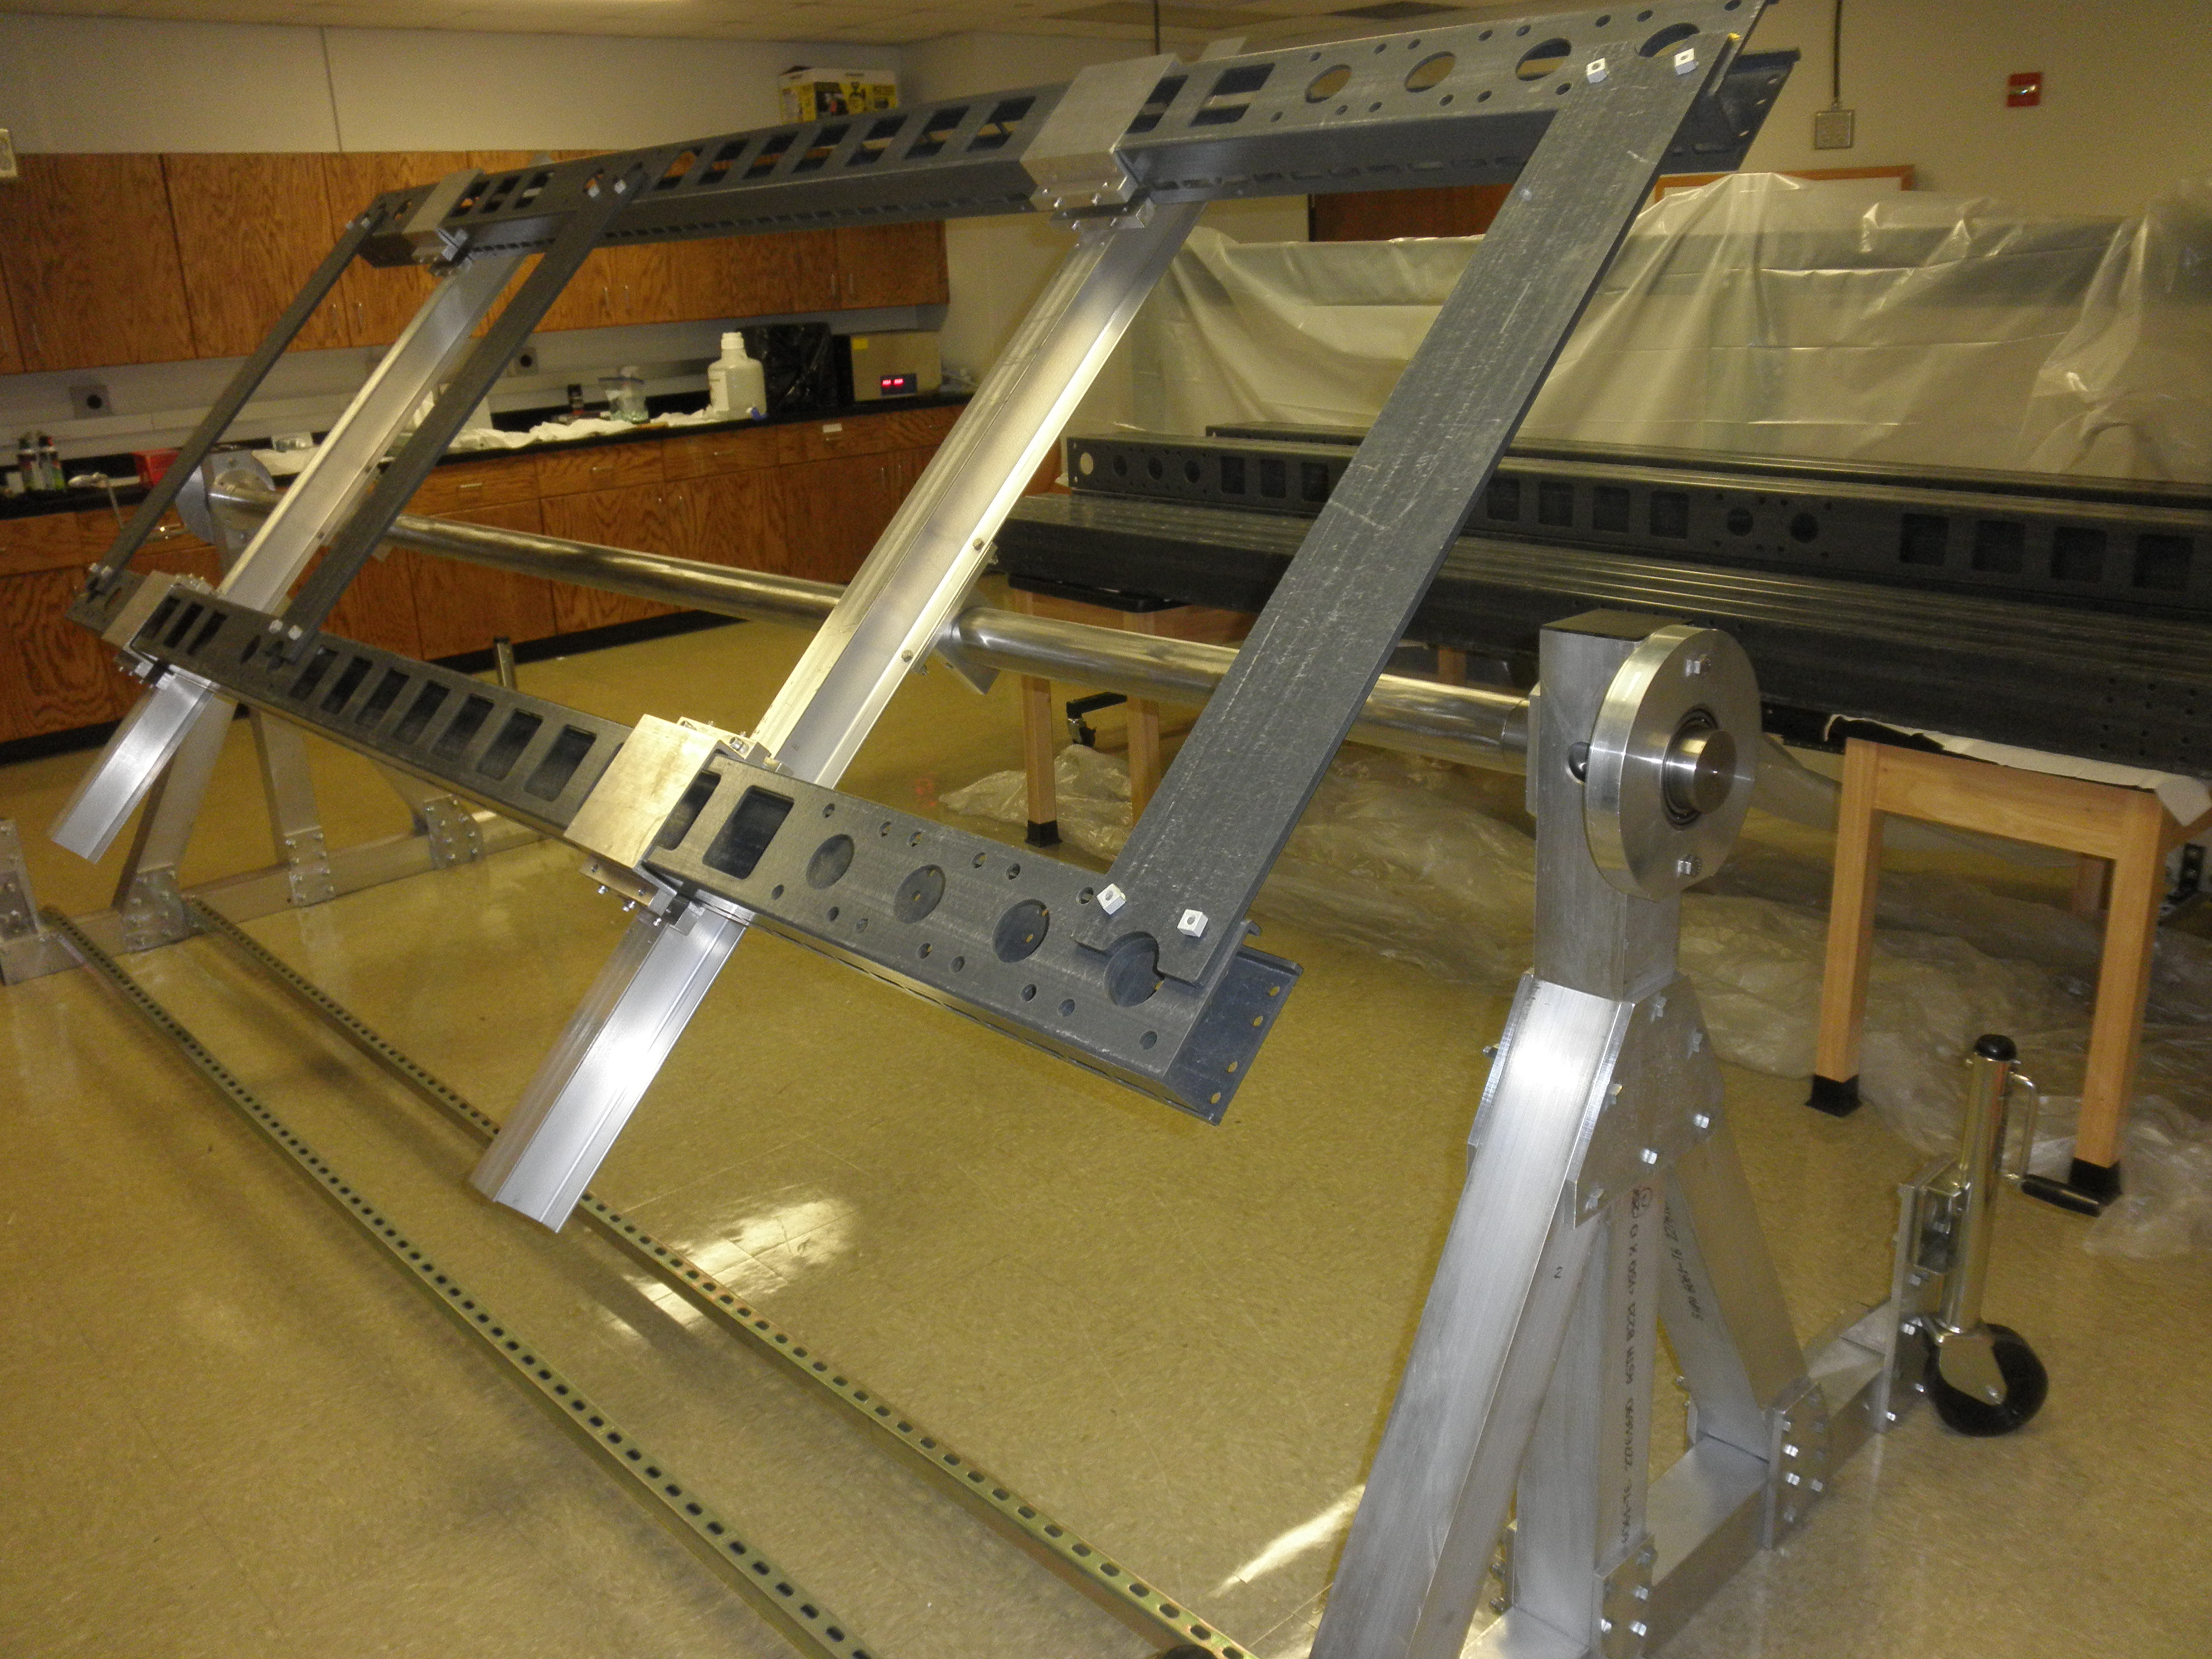
\includegraphics[width=0.8\textwidth]{endwall_assy_rot_table}
 \end{dunefigure}
 
The FRP box beams are sandwiched between 1.3 cm (1/2 inch) thick FRP panels which are held on one side by means of G10 bushings and rods with square nuts
as shown in Figure \ref{fig:endwall_assy_detail}. One the other side M10 stainless steel bolts engage with large slip nuts that are inserted into the Al profiles. The profiles 
are pulled towards a 2.5 cm thick FRP plate (red in Figure \ref{fig:endwall_assy_detail}) on the inside of the box beam.

\begin{dunefigure}[Endwall Assembly Side Detail]{fig:endwall_assy_detail}{ Left: Side view of upper part of a FC endwall top module. The left side shows FRP bushings and rods held by square nuts whereas the right side of the panel shows the M1o stainless steel bolts which engage in slip nuts inserted into the Al profiles. Right: Top module and baseline field cage endwall module frames hanging.}
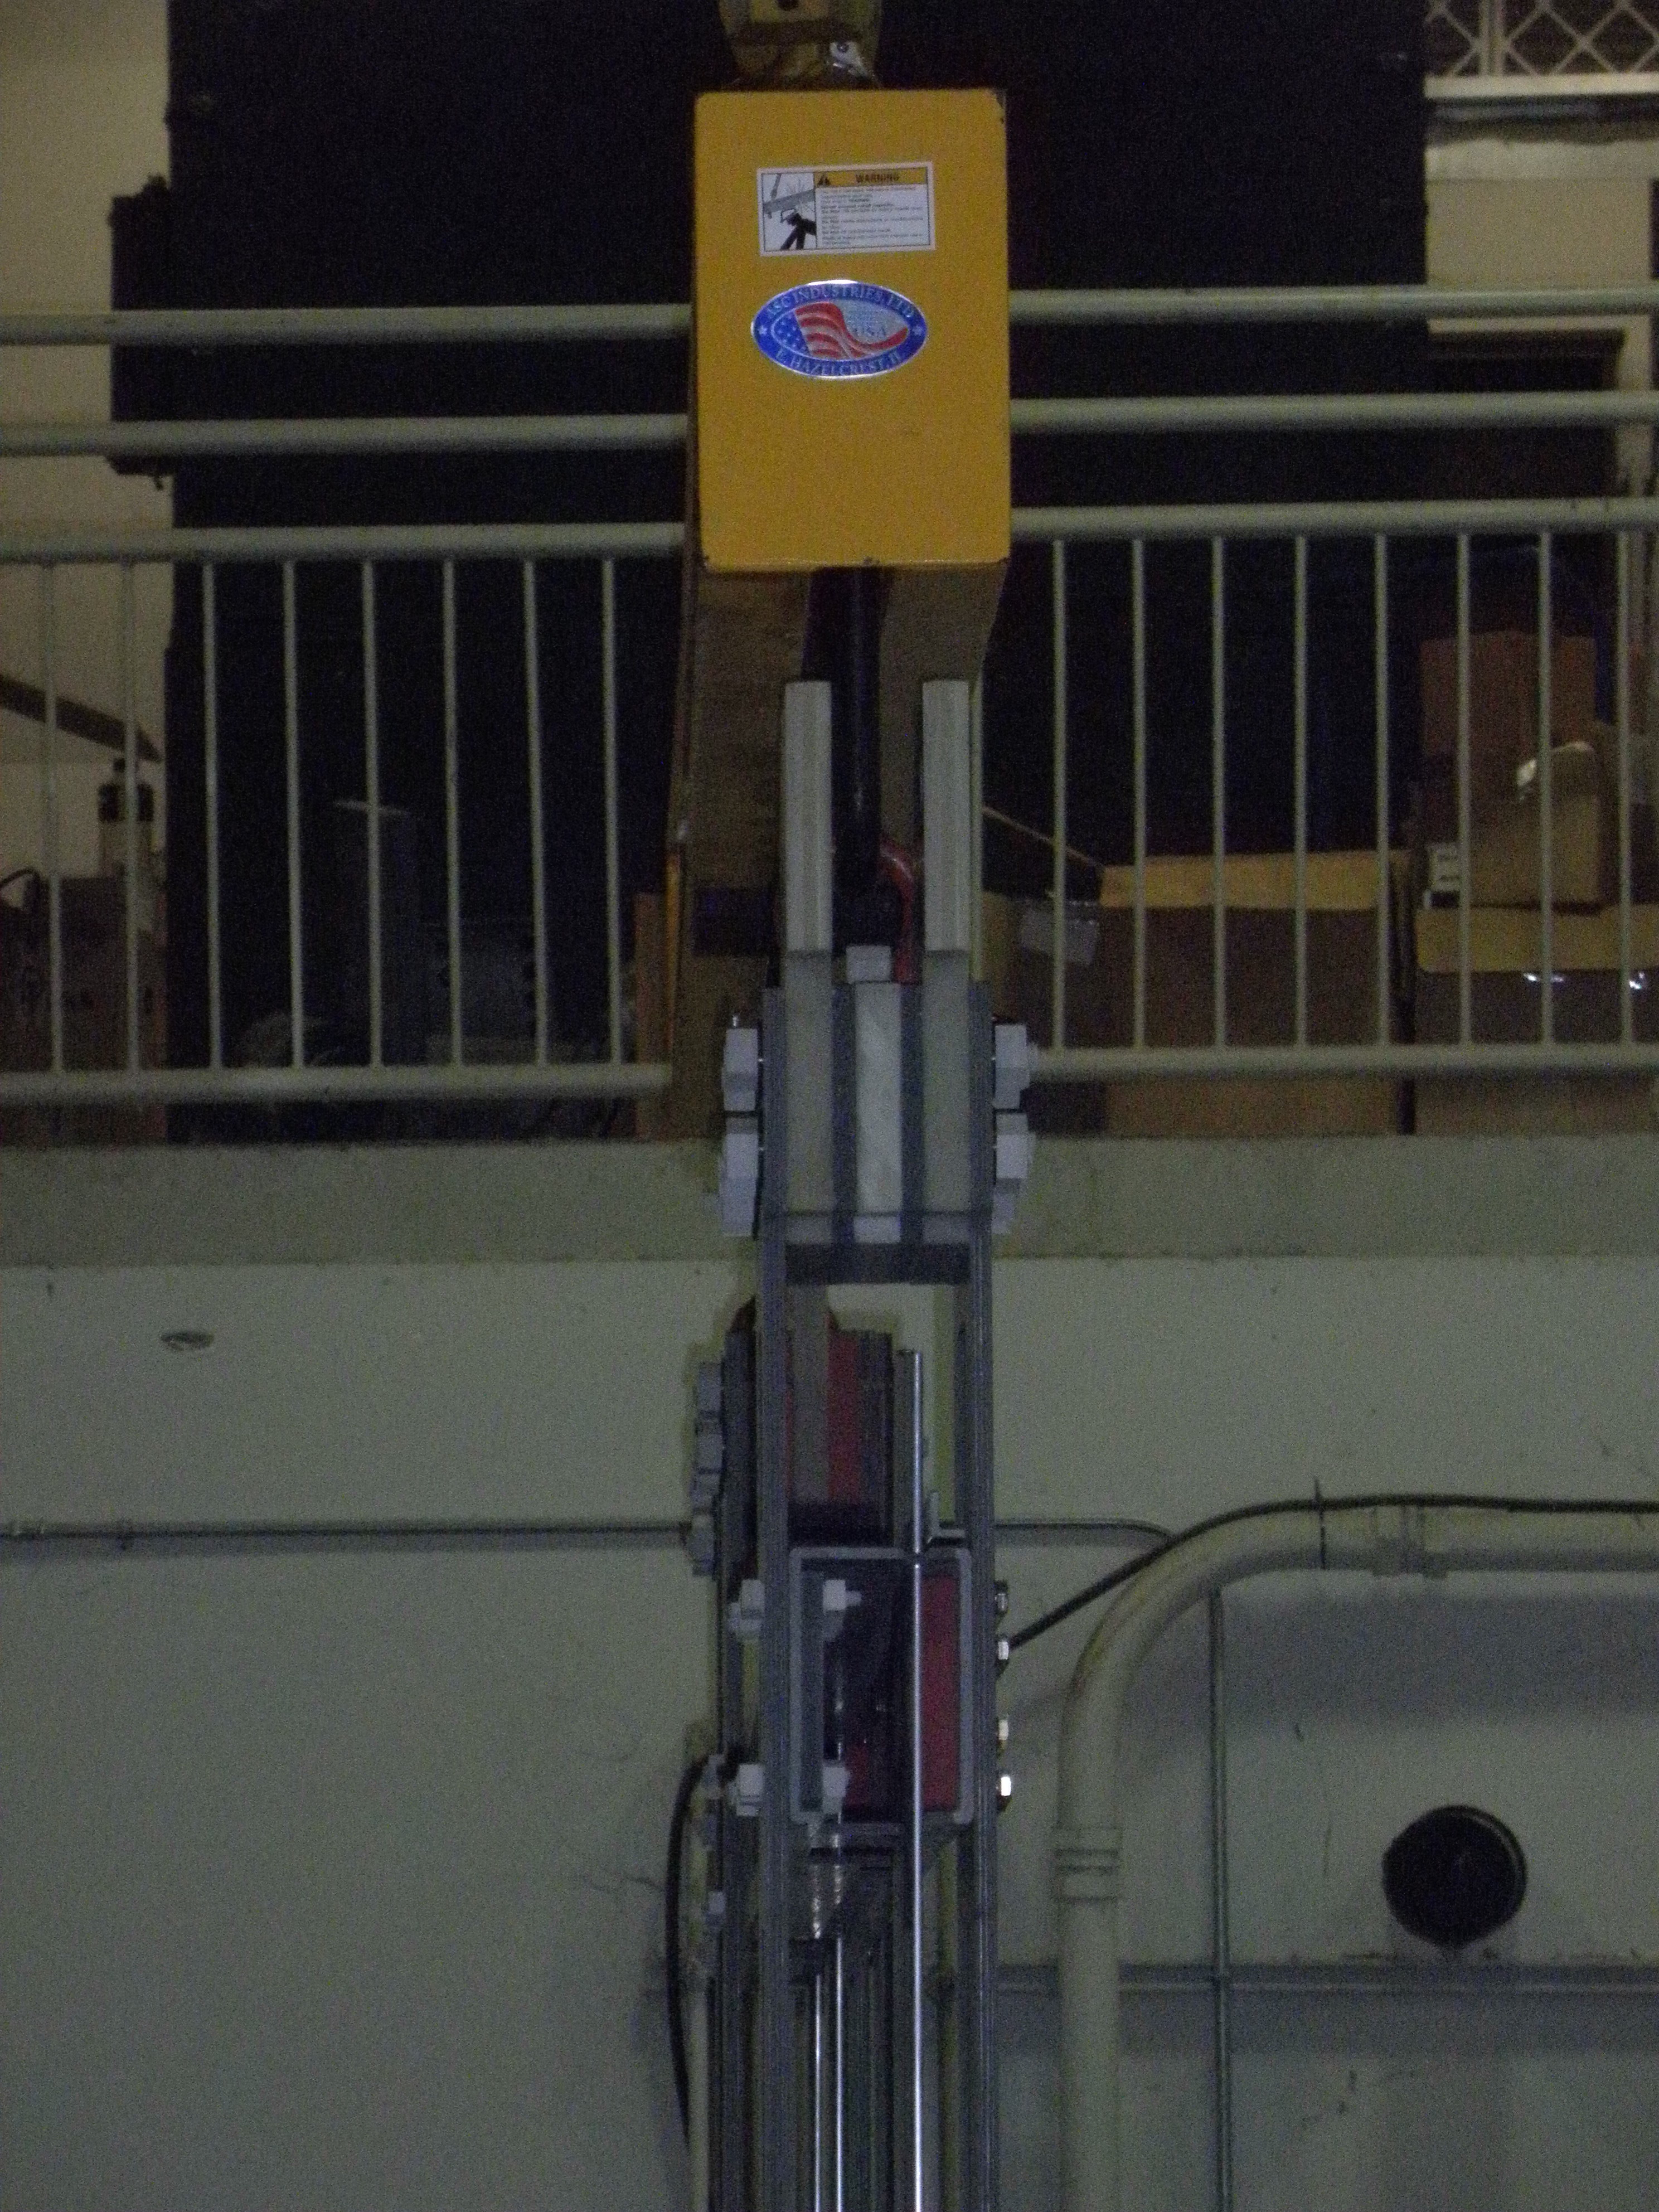
\includegraphics[width=0.48\textwidth]
{fc_endwall_detail_side}
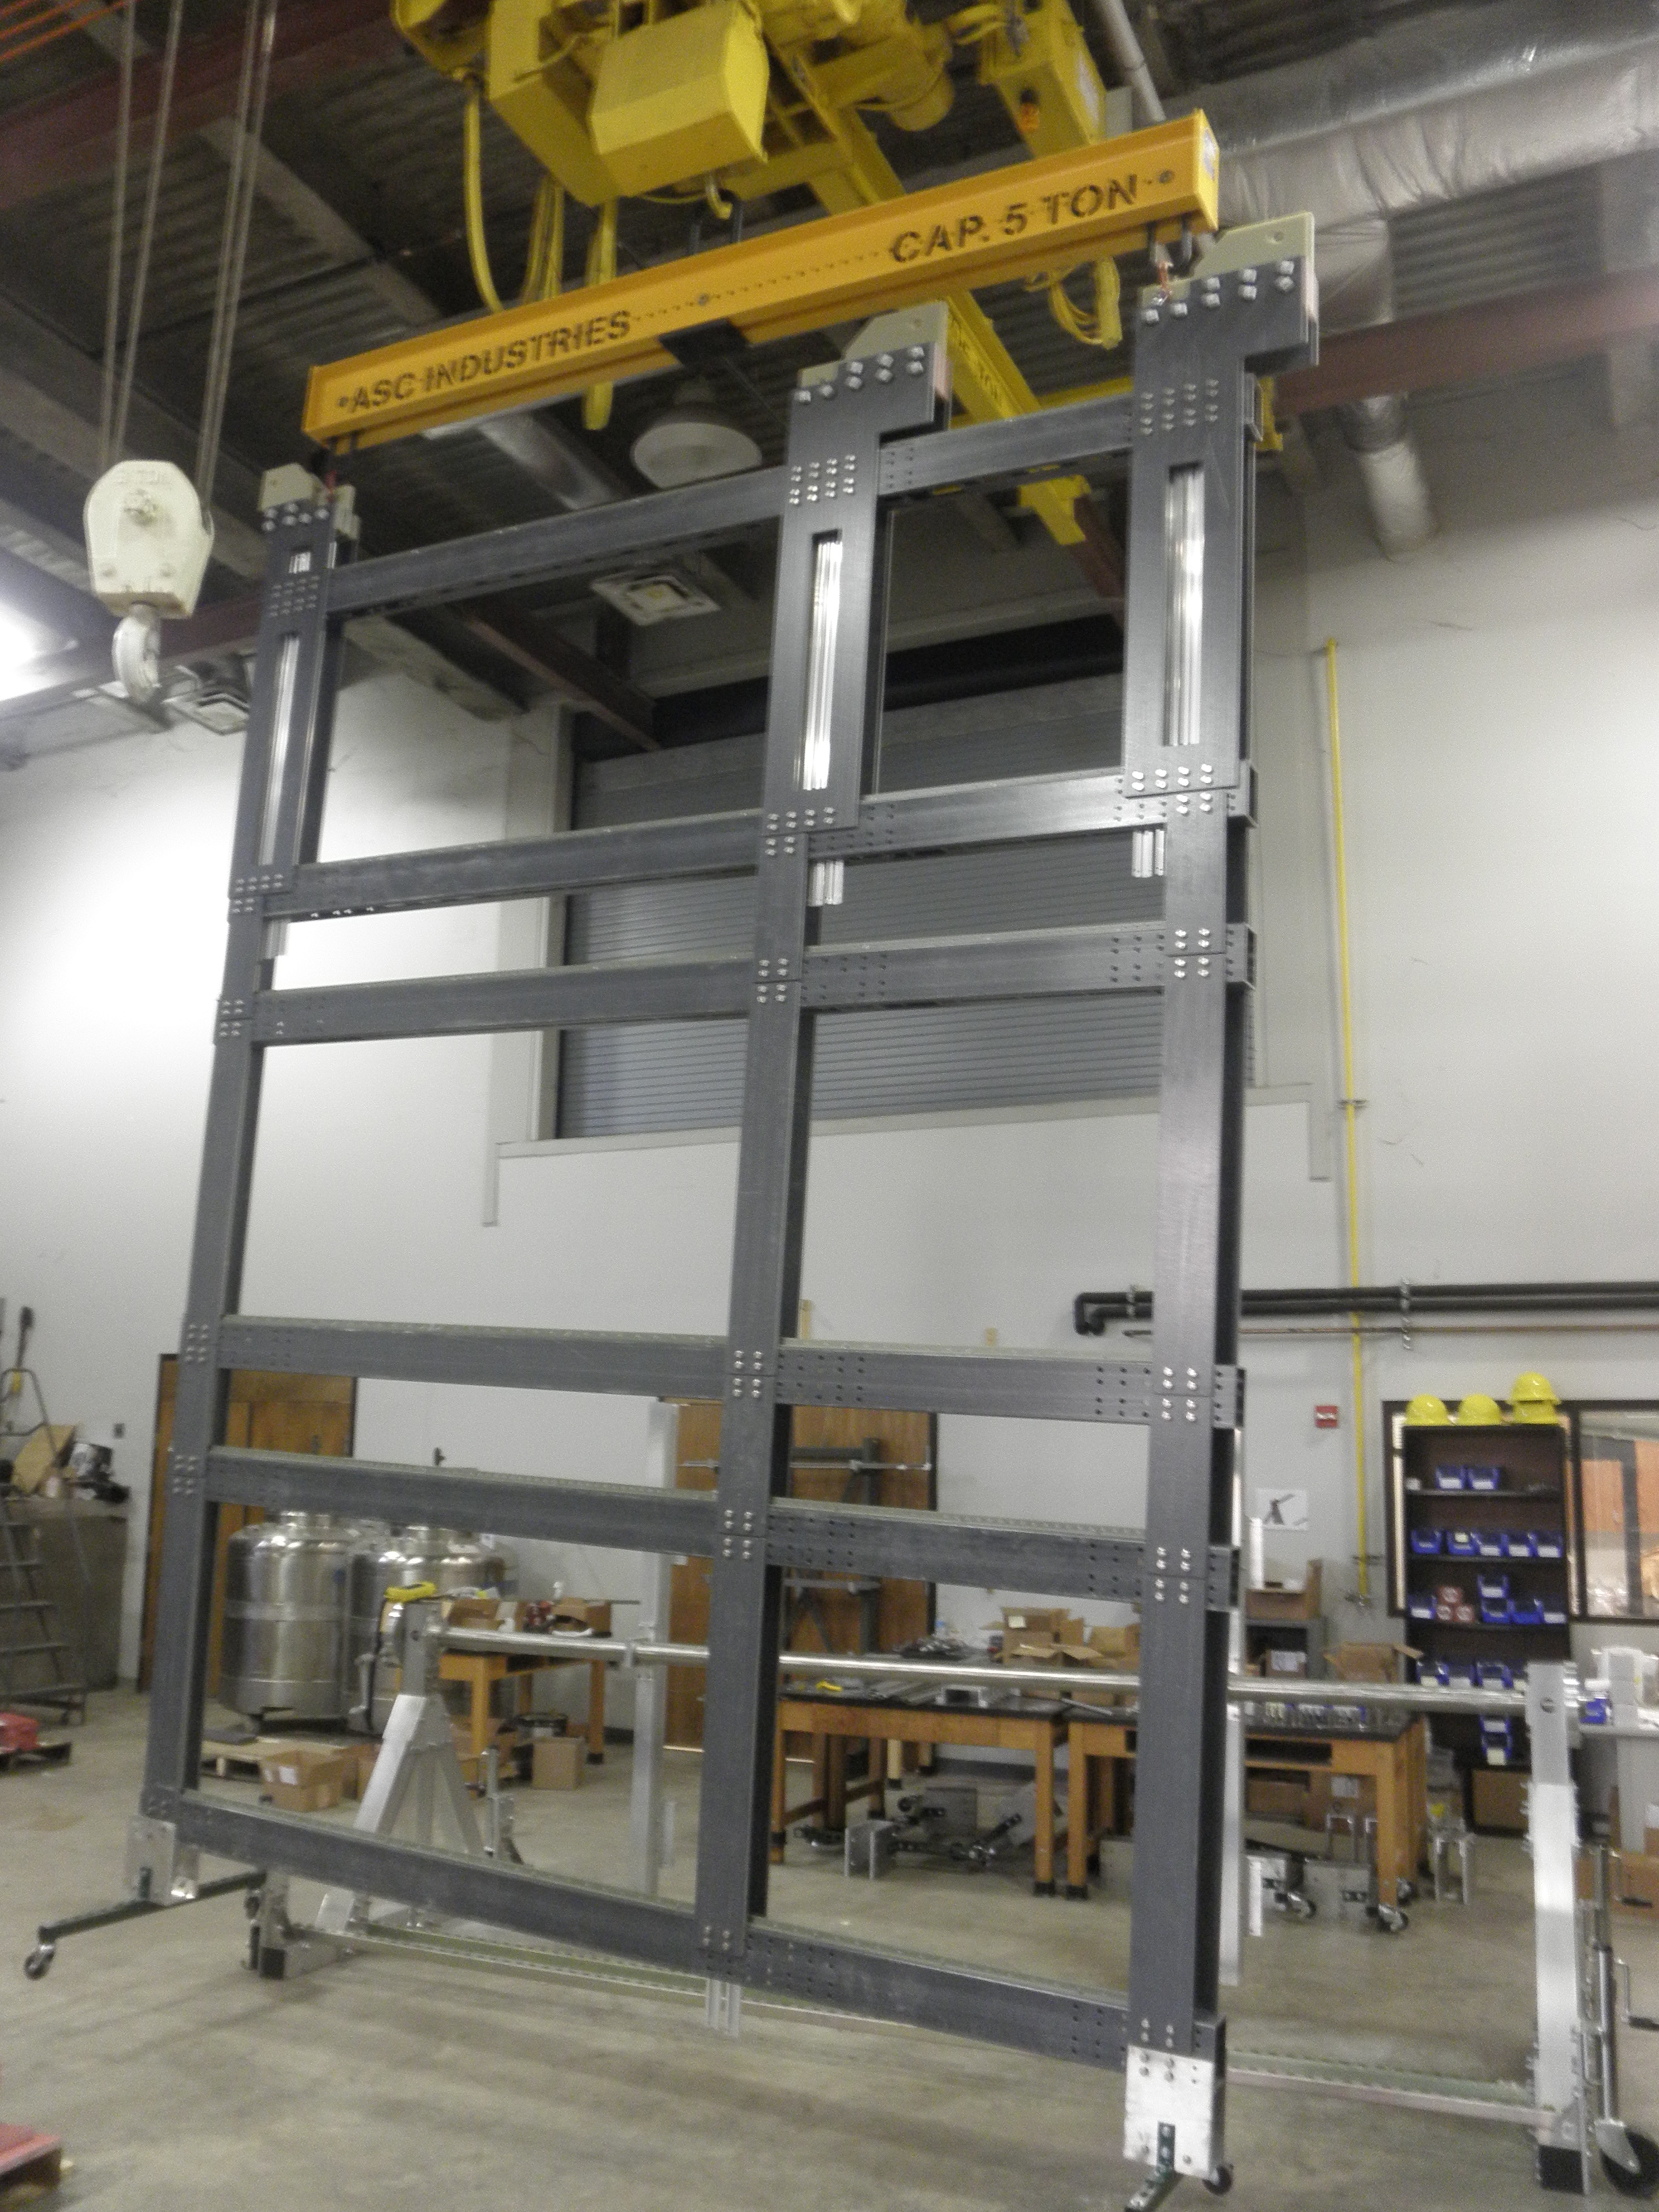
\includegraphics[width=0.48\textwidth]
{3_fc_endwall_frames_hanging}
\end{dunefigure}

Aluminum profiles are inserted into the cutouts of the box beams and attached with screws and stainless steel slip nuts to brackets that are mounted on the 
FRP box beams. After this, the resistive divider boards are mounted to the profiles using brass screws that engage with stainless steel slip nuts inside 
the profiles.

\subsection{Electrical Interconnections}
\label{sec:fdsp-hv-prod-interconnect}

All electrical fasteners and wires used on the CPA and FC will be produced
to specification by commercial vendors and packaged with the CPA or FC modules.  
As discussed above (\ref{sec:fdsp-hv-prod-cpa}, \ref{sec:fdsp-hv-prod-fc}), 
this includes the HV cable segments, as well as wire jumpers, machined brass
tabs, etc.

Circuit boards for DUNE HV interconnections will be produced and tested at the  university shops according to the same design used for ProtoDUNE.  The FC voltage dividers were produced for ProtoDUNE at Louisiana State University, and the boards for CPA Frame bias and CPA-FC connections were produced at Kansas State University.
%\todo{What about the FC-to-APA boards?} 
Both institutions have created custom test apparatus for verifying proper operation of the boards at full voltage and over-voltage conditions.  Production and testing could be
scaled up by the required order of magnitude at these institutions, or shared with
other institutions, whichever best meets the needs of the project.
Each board will be free of solder flux and flux-remover. 


%%%%%%%%%%%%%%%%%%%%%%%%%%%%%%%%%%%%%%%%%%%%%%%%%%%%%%%%%%%%%%%%%%%%
%\section{Interfaces (Bo)}
%\label{sec:fdsp-hv-intfc}
%
%%%%%%%%%%%%%%%%%%%%%%%%%%%%%%%%%%%
%\subsection{Interfaces to APA}
%\label{sec:fdsp-hv-intfc-cpa-fc}
%
%
%%%%%%%%%%%%%%%%%%%%%%%%%%%%%%%%%%%
%\subsection{Interface to DSS}
%\label{sec:fdsp-hv-intfc-dss}
%
%
%%%%%%%%%%%%%%%%%%%%%%%%%%%%%%%%%%%
%\subsection{Interface to PDS}
%\label{sec:fdsp-hv-intfc-pds}
%
%%%%%%%%%%%%%%%%%%%%%%%%%%%%%%%%%%%
%\subsection{Interface to CE}
%\label{sec:fdsp-hv-intfc-ce}
%
%%%%%%%%%%%%%%%%%%%%%%%%%%%%%%%%%%%
%\subsection{Interface to Calibration}
%\label{sec:fdsp-hv-intfc-cal}
%
%
%
%%%%%%%%%%%%%%%%%%%%%%%%%%%%%%%%%%%%%%%%%%%%%%%%%%%%%%%%%%%%%%%%%%%%
\section{Installation, Integration and Commissioning}
\label{sec:fdsp-hv-install}

%%%%%%%%%%%%%%%%%%%%%%%%%%%%%%%%%%%%
\subsection{Transport and Handling}
\label{sec:fdsp-hv-install-transport}

The power supply, cables, filters, and feedthroughs will be sent to the site in standard shipping crates.  Handlers will wear gloves when handling insulators that will be between high voltage and ground.  Surfaces can be cleaned with alcohol and allowed to dry.

CPA-Panels will be shipped in crates to the SURF site.  The 12 m CPA-Panels will be disassembled into their three CPA-Units, loaded into the crates with all hardware needed to complete the CPA-Panel assembly at the SURF site.  Each shipment should consist of two crates which contain the two CPA-Panels that will be paired to form a CPA-Plane. There will be very little room for storage at the SURF site, so it is important to ship CPA-Panels in this way so that final assembly, integration, and installation can proceed as soon as components are received.

Top and bottom (T/B) field cage modules will either be fully assembled at University production sites and shipped to SURF ready for installation into the mine, or the components will fabricated and QC inspected at University sites before being shipped to SURF for final assembly, as was done for the ProtoDUNE modules at CERN. Crate design for T/B modules will depend strongly on whether the ground planes remain attached to the modules, as in the ProtoDUNE design, or if the ground planes are, instead, connected directly to the cryostat. In the former case, if fully assembled T/B modules with attached ground planes are transported into the mine, the complexity of the crates will be significantly enhanced, as it is difficult to fully support a module on all sides while allowing for tipping of the crate. Hence, it may be necessary for ground planes to be installed underground in either design scenario. Thus far, only single fully assembled T/B modules have been crated for shipment, but more complex designs that will allow for multiple modules (without installed ground planes) will be developed.

Endwall Transport and Handling:

The end wall sections each consisting of eight modules are each shipped in separate shipping crates are layered sequentially with the bottom piece on the top of the crate.  They are unpacked as follows:

\begin{itemize}
\item Unpack FC Endwall modules from crate one at a time. 
\item Attach spreader bar to the  top mounting plate of a single panel.
\item Carefully remove outer plastic bag while frame is hanging freely.
Crane panel onto assembly table and rotate into horizontal position using the ledge on the assembly table to prevent panel from sliding. 
(Steel bolts should be on top when frame is in horizontal position).
\item Remove spreader bar. Position correctly in assembly area.
\item Remove inner plastic bag carefully not to damage any parts of a FC Endwall module.
\end{itemize}

HV bus segments, FSS bias boards, and  interconnection wires will be integrated with the CPA-Units before shipment, while CPA-panel interconnections and FSS connection tabs will be packaged and shipped with the CPA-Panels for integration on site.
FC divider boards will be attached to FC modules during FC assembly as described in \ref{sec:fdsp-hv-prod-fc}.
The CPA-to-FC and FC-to-APA boards will shipped separately and attached just before each FC is hoisted onto its CPA-Panel in order to avoid risk of damage to exposed boards on the ends of the FCs during shipment and handling.


%%%%%%%%%%%%%%%%%%%%%%%%%%%%%%%%%%%
\subsection{Installation and Integration}
\label{sec:fdsp-hv-integration}
Upon arriving at the DUNE site, The CPA shipping crate is unpacked with the Middle/Lower CPA-Unit placed in a vertical stand on the floor of the ``toaster'' region.  Next, the Middle/Middle CPA-Unit is removed and vertically attached to the Middle Lower Unit.  Finally, the Upper/Middle CPA-unit is removed and attached.  This assembly makes up a CPA-Panel.  The CPA-Panel is lifted and vertically attached to its trolley with a FR4 hangar.  Two CPA-Panels are paired to form a CPA-Plane which then forms the unit for attachment of the FCs.  Figure~\ref{fig:cpas-in-cryostat} shows on the left a 2-Panel CPA-Plane mounted on its trolleys in the clean room at ProtoDUNE, waiting for installation of the Top and Bottom FC units.

It should also be noted that the CPA-Panels on each end of each CPA-Array are special - they have aluminum profiles along the exterior side to form the first element of the field cage.  They also contain parts of the HV Bus mounted on the CPA frames.  The HV Bus forms a continuous loop from the HV Input through the top of the 25 CPA-Planes, down the far external side, back along the bottom and up the  external side back to the HV Input.

\begin{dunefigure}[ProtoDUNE CPA Plane before and after FC attachment]{fig:cpas-in-cryostat}{Left: Completed ProtoDUNE CPA-Plane ready for FC attachment. Right: Two completed CPA/FC assemblies in the ProtoDUNE SP cryostat.}
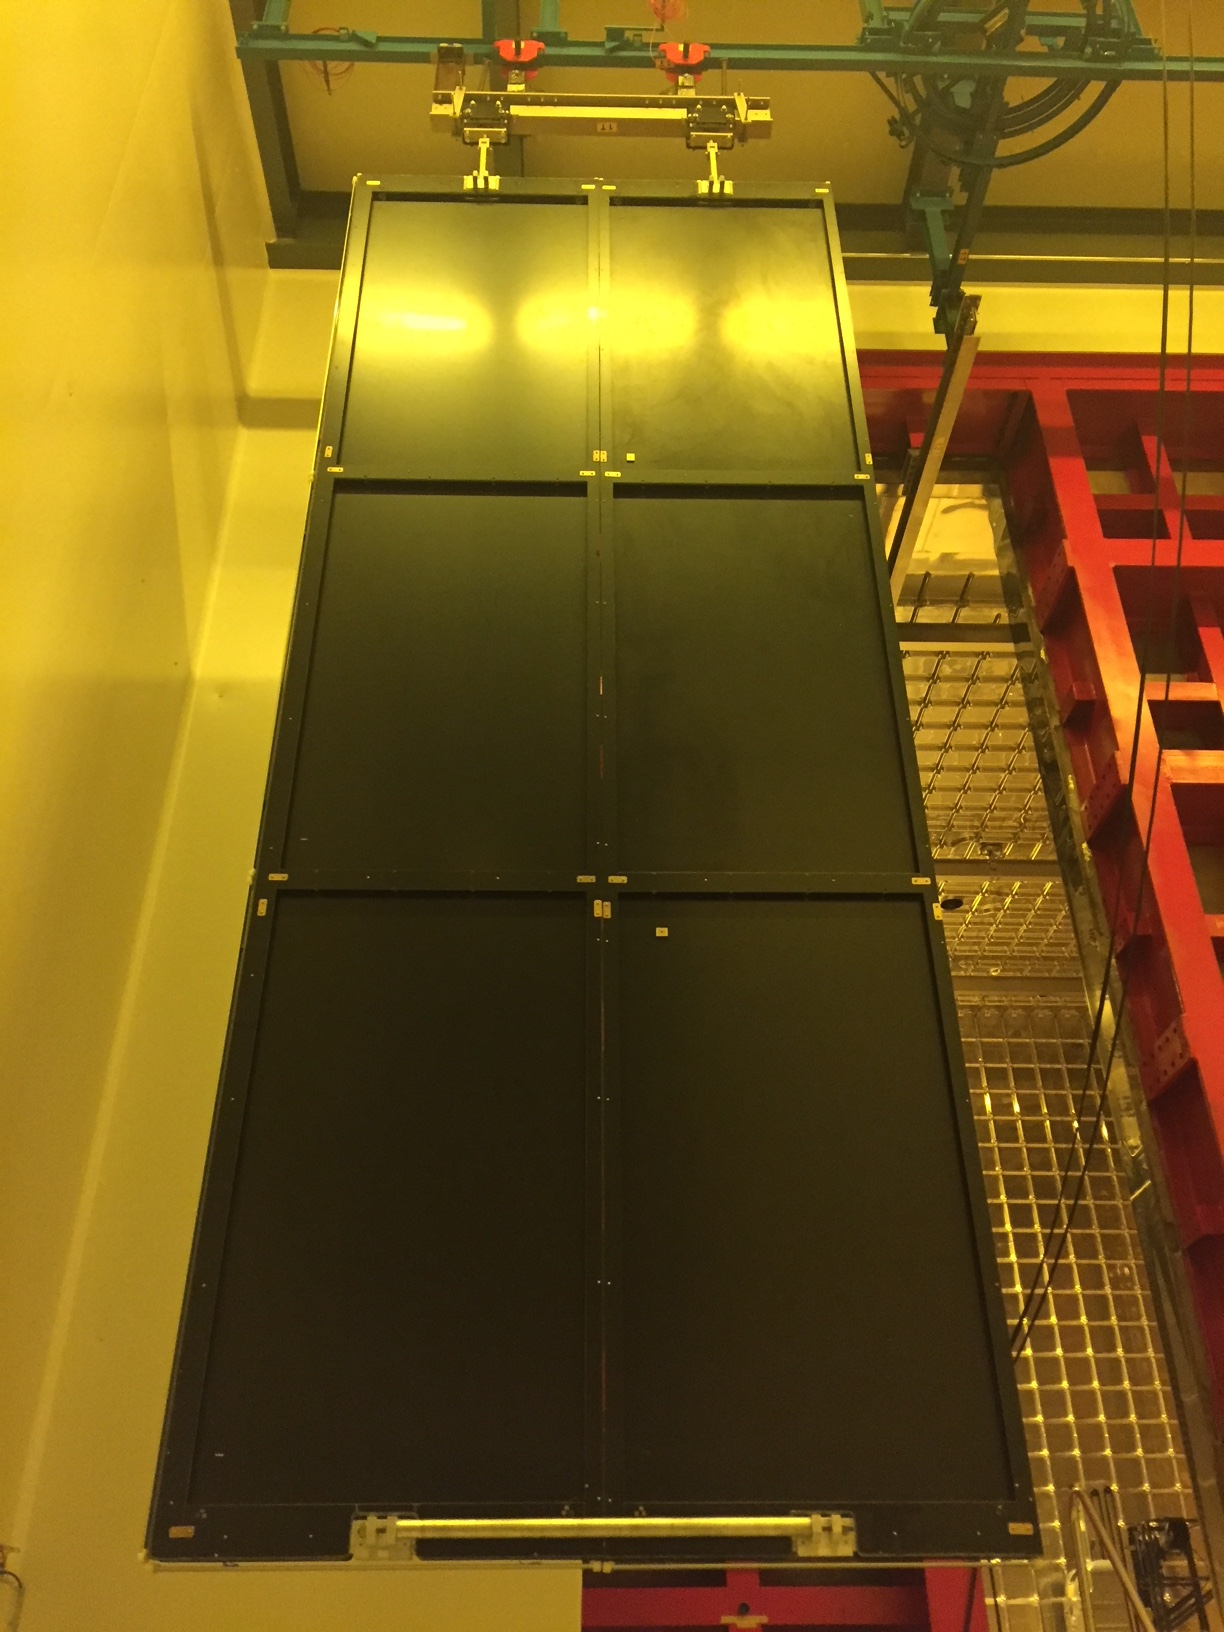
\includegraphics[width=0.45\textwidth]{lastcpa}
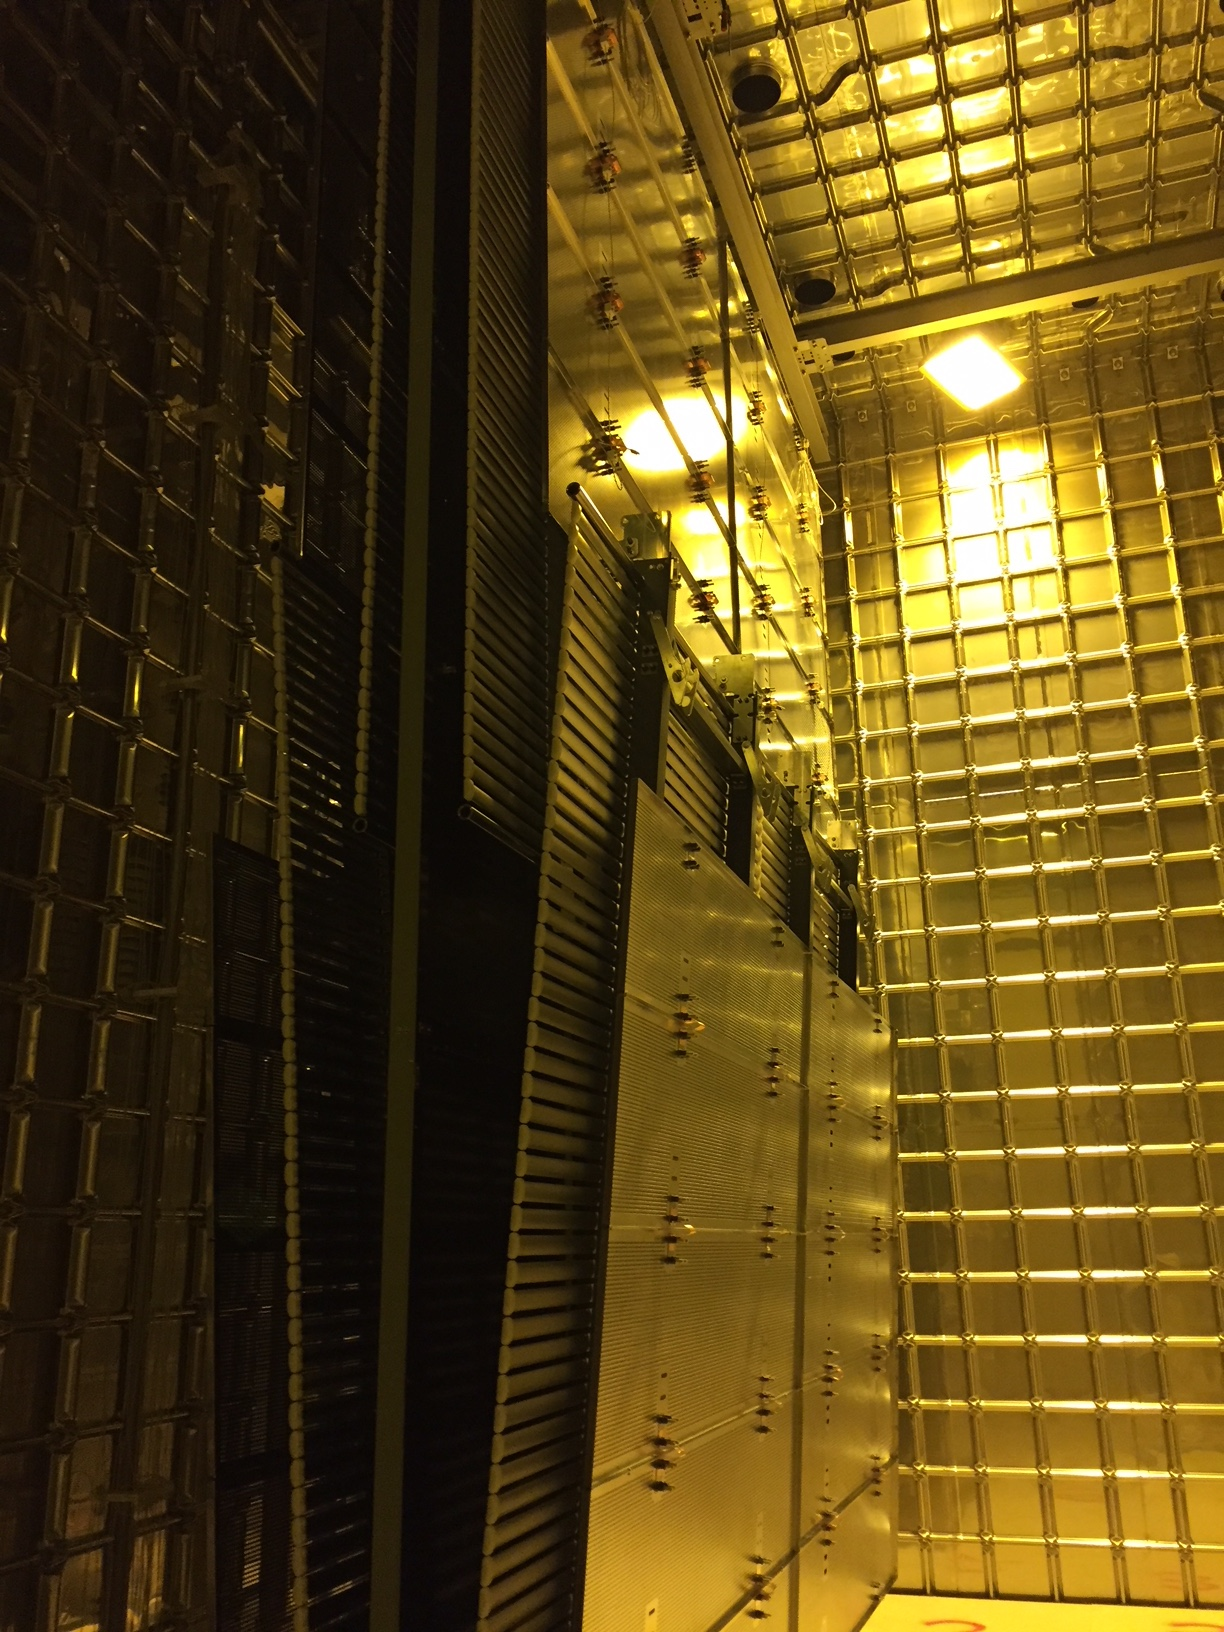
\includegraphics[width=0.45\textwidth]{2cpas-in-cryostat}
\end{dunefigure}

There are a total of 50 CPA-Panel pairs (CPA-Planes) arranged in the DUNE cryostat in two rows of 25 each.  After the Panels are paired, FC units are attached folded against the CPA and the full CPA/FC assembly is placed in the DUNE cryostat through the access door.  Figure~\ref{fig:cpas-in-cryostat} shows on the right two completed CPA/FC assemblies on their beam in the ProtoDUNE SP cryostat.


Upon deployment of the folded Top and Bottom FC units, and after the final Endwall installations, the TPC field cage is complete.

To assemble the Endwall EW-FC, the modules are rotated vertically in the assembly area, then placed in a stand designed to hold the 120kg pieces vertically.

The top module is lifted and moved above the next module in the vertical stand where the two are bolted together and any electrical connections are made. The two modules are then lifted up and aligned above the following module.  The modules are again bolted, electrically connected and it is raised and aligned above the next piece.  This process is repeated until all 8 modules are hanging together.  Once the bolting and electrical connections have been completed on the last piece the continuity of all the grounding connections of the end wall are checked.
 
The completed end wall section is then moved over to the installation beam where its spreader bar is attached to the installation system.  It is then rolled into the cryostat and located on the appropriate beam for installation into the TPC.

\begin{dunefigure}[ProtoDUNE Endwall Installation]{fig:EndwallInstall}{Completed Endwall in process of installation into ProtoDUNE SP cryostat}
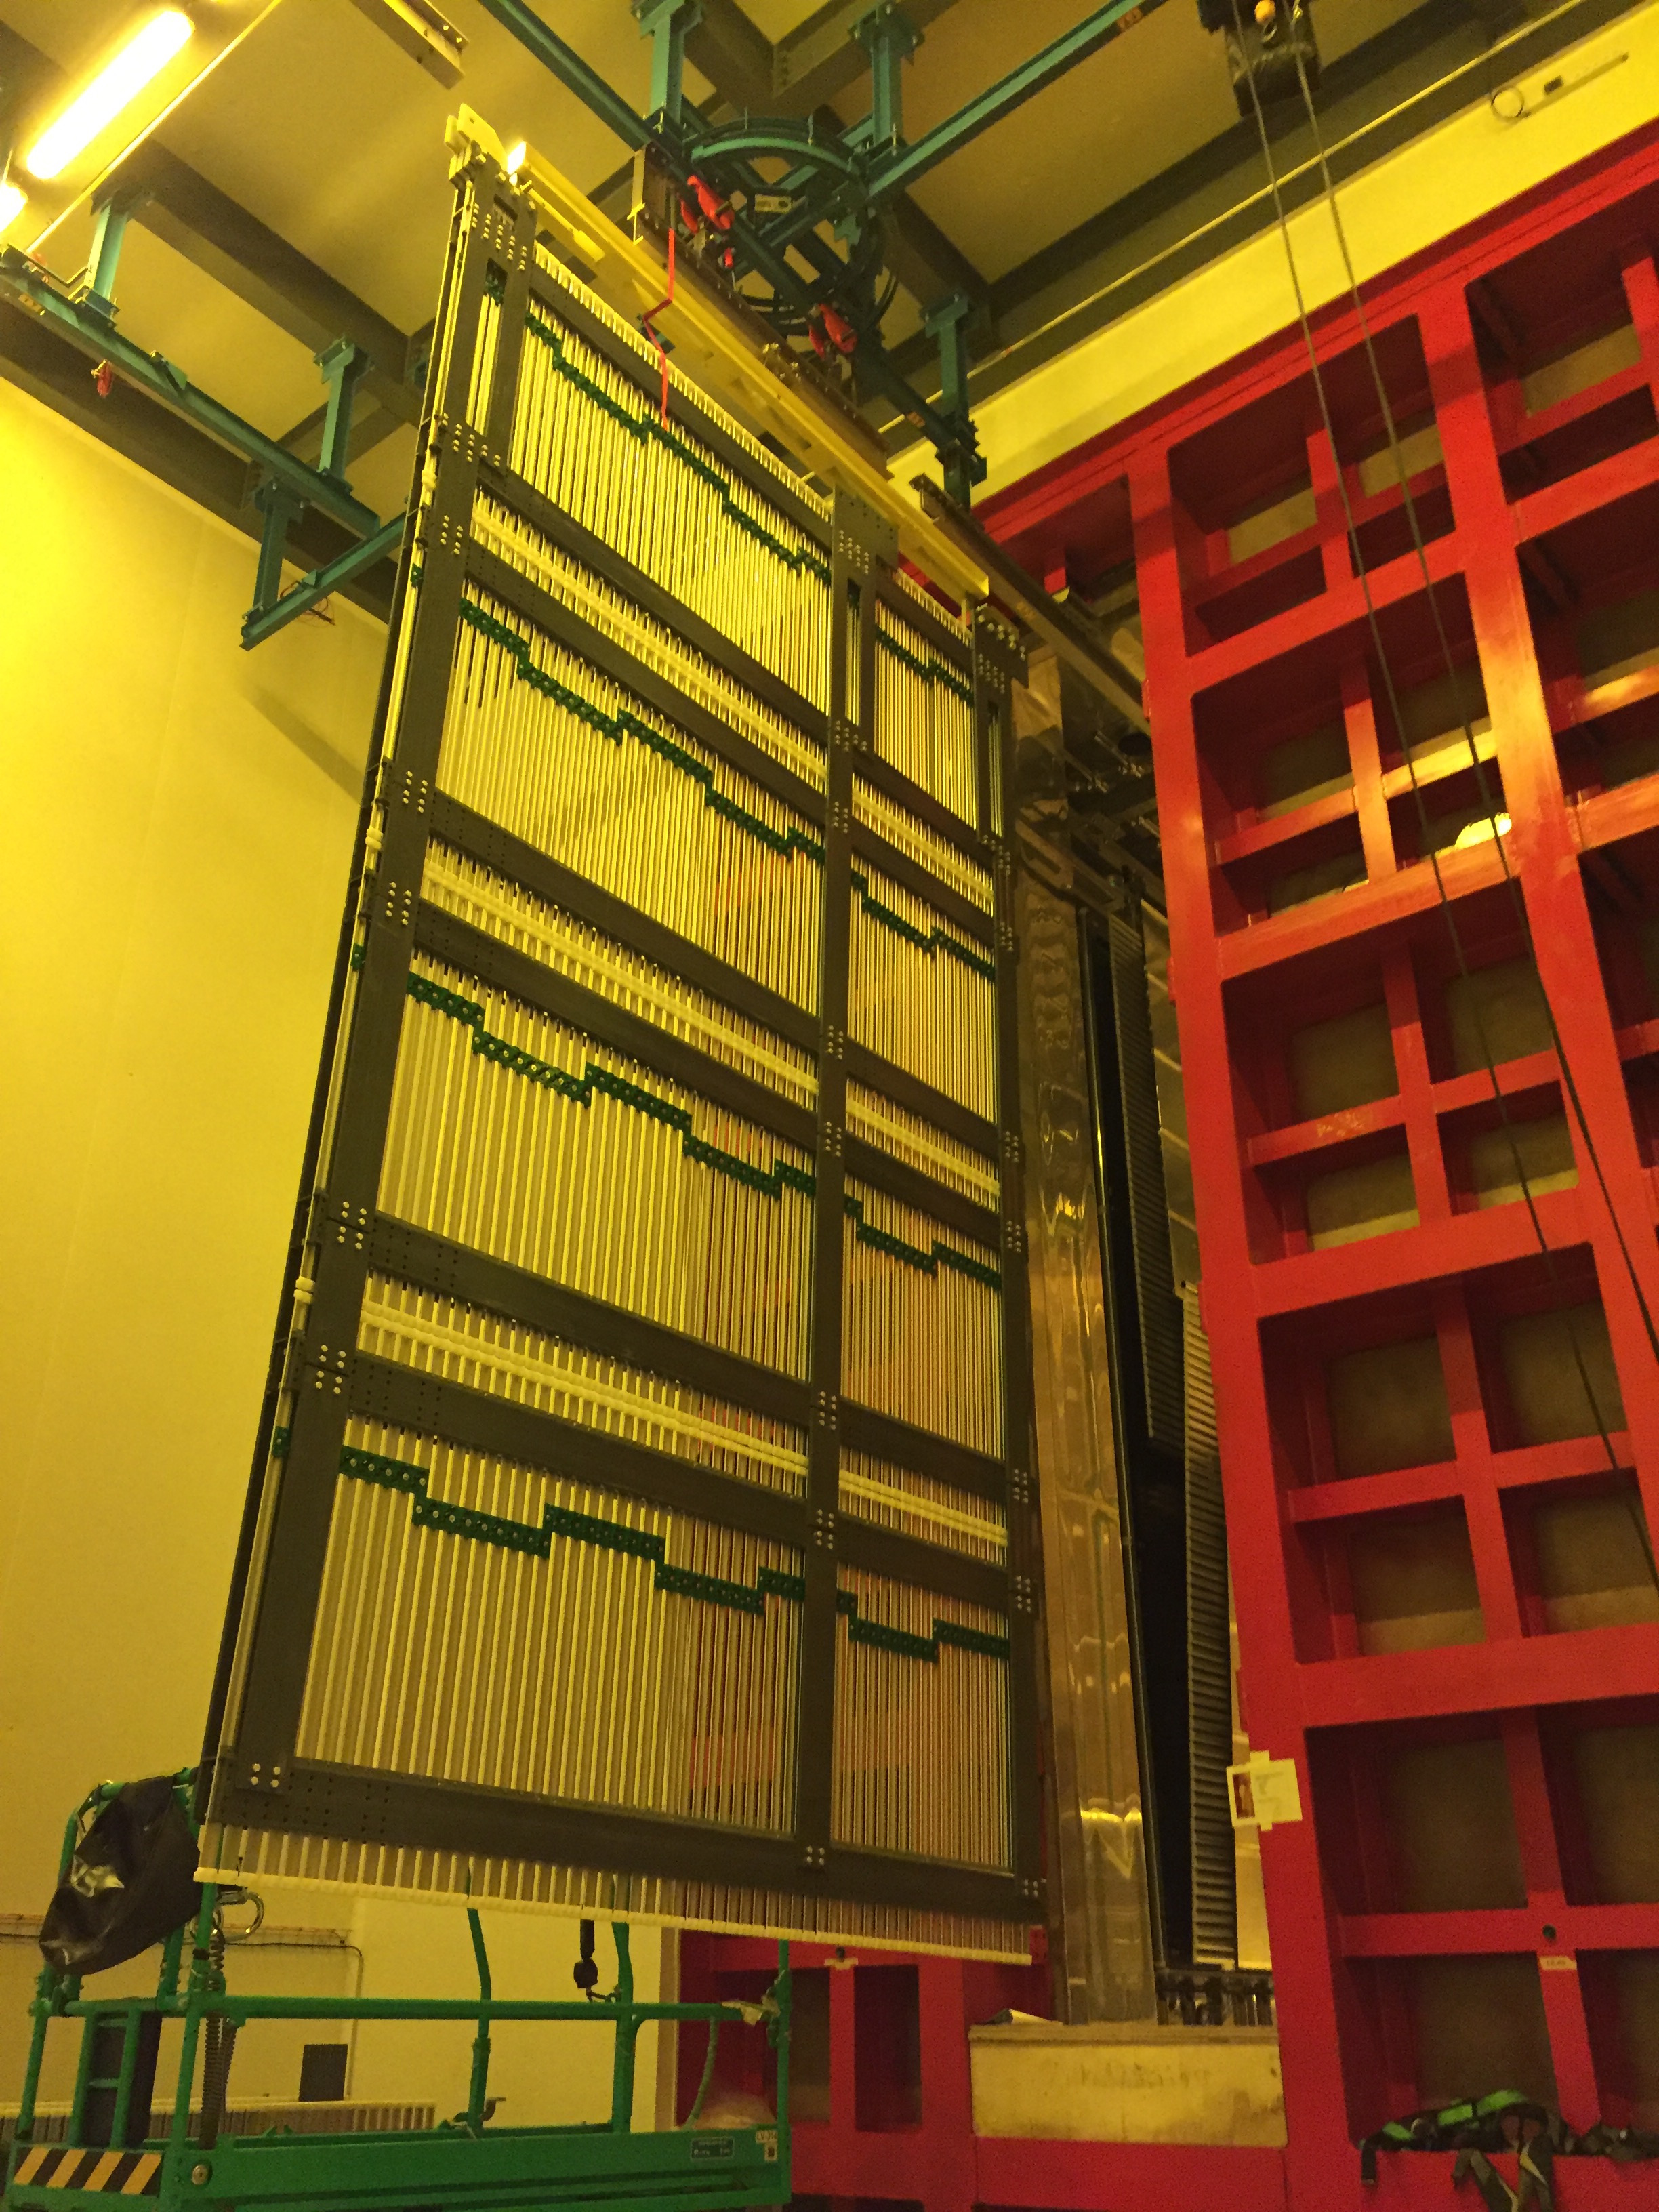
\includegraphics[width=0.45\textwidth]{endwall_and_tco.jpg}
\end{dunefigure}



\subsection{Interfaces}
\label{sec:fdsp-hv-interface}

Among TPC components there are internal interfaces between the CPA and FC; the CPA and HV, and  the FC and HV. In addition there are significant interfaces with systems from other Consortia.

The interfaces with the high voltage system include the electrical connections with the HV cup, HV bus, and field cage, interconnect the panels within the CPA, and propagate the HV bus between adjoining CPAs.  A selection of the mechanical interfaces are as follows:
\begin{itemize}
\item Metal contact plates on the cathode surface at each corner, with two captive screws in each used for making electrical contact with the HV bus and the resistor board for the frame field strips
\item Through holes for the 3-mm diameter cable in the sides of each frame adjacent to the contact plates to allow interconnection of the HV bus between CPAs.
\item A means of securing the HV bus cable in place.
\item Through-holes near the centers of the top and bottom frames for connecting the top and bottom field cage elements to the cathode, with corresponding metal contact plate on the cathode surface
\item Electrical specifications for these parts and interfaces are given in the High Voltage Design Section
\item Between the CPA and the FC the interface is at the hinge joint and insuring that the CPA and FC are located relative to each other properly.
\end{itemize}

Since these interfaces occur with the design group that is constructing the TPC there is close coordination and communication between the CPA, FC and HV groups to ensure that all requirements are met and that the components all fit together.  

The interfaces between the CPA system and the HV system, and the interfaces among the CPA/FC/HV systems are shown in integration drawings and documented in the project documentation system.

%DUNE-3 is a drawing that is used to define the interface between the CPA system and HV system and DUNE-6 is an integration drawing that defines the interface between the CPA/FC/HV systems.  These drawings can be found in DocDb 1870. 

The various components in the HV System also have interfaces with components from other systems.  These interfaces are formally defined by interface documents. Detailed descriptions of major interfaces in DUNE can be found (here?). Key interfaces between the HVS and other systems are summarized in Table~{\ref{tab:hvinterfaces}} below:

%The external interfaces and defining DOCDB number are listed in the table below.


%Interface	DOCDB 
%TPC with Cryostat	1677
%TPC with Detector Support Structure	1681
%TPC with Photon Detection System	1682
%TPC with DAQ/Computing/Slow Controls	1683
%TPC with Rack Space and Power Requirements	1684



\begin{dunetable}
[HV System Interfaces]
{p{0.2\linewidth}p{0.75\linewidth}}
{tab:hvinterfaces}
{Key HV System Interfaces to Other Systems} 
Interface to & Description \\ \toprowrule
DSS  &  Support, positioning, and alignment of all CPA, FC modules inside the cryostat both warm and cold\\ \colhline
APA & Field cage support (top, bottom, and end wall) on APA frames; Mounting of field cage termination filter boards and FC failsafe terminations; Mounting of the Electron Diverter boards.
\\ \colhline
TPC Elec. & Field cage termination wire connectors on CE feedthrough flange, FC termination wires routed with CE cables
 \\ \colhline
PDS & Mounting of PD calibration flash diffusers and routing of their fibers on CPAs; TPC coated reflector foil on CPAs (TBD).
 \\ \colhline
Facility & Locations and specifications of the HV Feedthrough ports; gas and liquid argon flow velocities and patterns. \\ \colhline
Calibration & Field cage openings for the calibration laser heads \\ \colhline
Cryo. Inst. \& Slow Ctrl. & HV vs. LAr level interlock, sensor locations in high field regions, cold/warm camera coverage, HV signal monitoring, etc. 
 \\ \colhline
Integr. Facility & Storage buffer, inspections/tests, repackage for  underground delivery
 \\ \colhline
Physics / Software & Requirements: range of operating drift field, uniformity of the drift field; Supply detector geometry and E field map.
 \\ \colhline
\end{dunetable}

%%%%%%%%%%%%%%%%%%%%%%%%%%%%%%%%%%%%%%%%%%%%%%%%%%%%%%%%%%%%%%%%%%%%
\section{Quality Control}
\label{sec:fdsp-hv-qc}

Power supplies used in DUNE will be tested before installation.  Output voltages and currents must be checked on a known load. 

The feedthrough and filters should be tested at the same time, preferably with the planned power supply.  The feedthrough must be tested to hold the required voltage in TPC-quality liquid argon ($\tau\geq$\SI{1.6}{ms}) for several days.  The ground tube submersion and electric field environment of the test setup should be comparable to the real field cage setup or more challenging ({\it e.g.}\ the test liquid level can be lower than DUNE's but not higher).  Additionally, the feedthrough must be leak tight to satisfy cryogenic requirements.

CPA QC consists of forms that are filled out as part of the various procedures from initial assembly at factories to the final testing of connections in the DUNE cryostat.  A group of QC forms filled out during initial Panel Unit assembly travels in the shipping crate with the Panel.  At SURF, Panel and Plane assemblies have their own set of QC forms for CPA assembly and for CPA/FC integration.  Finally, before Top and Bottom FC deployment, a final check of all electrical connections on the CPA and between the CPA and the Top, Bottom, and EndWall FCs is completed.  All of these forms are documented and available in the DUNE Document Database.

Before shipment of Top and Bottom Field Cages, each FRP component is subjected to inspection prior to assembly. Each of the beams is checked for flatness, torsion, and structural and surface defects, such as cracks or fractures, layer separation, thermal decomposition, and evidence of water-induced bloating. Any scratching or grooving of the surface layer can be remediated by coating with commercially available epoxy.

%%%%%%%%%%%%%%%%%%%%%%%%%%%%%%%%%%%%
%\subsection{During Local Production and Assembly}
%\label{sec:fdsp-hv-qc-local}

%QC Local for Endwalls
For the Endwalls, prior to assembly each box beam and all FRP stock will be inspected for dimensions, deformations, surface scratches and delamination defects. If the inspection is not passed, the parts will be rejected.
Preliminary assembly of EW-Modules will take place in a high-bay area under full crane access. After assembly, individual EW-Modules will be hung of each other in pairs of two to test the interconnections of the modules. Hanging will be performed in a top-down sequence consistent with space constraints (maximum 3 at once). This process will be repeated for all Endwalls. All parts will be labeled to uniquely identify their position. After disassembly, all parts are cleaned before being moved into the clean room, where they will be inspected again. Final assembly will occur in a dedicated clean laboratory space.

Each panel will undergo mechanical and quality control tests at LSU before shipping. Electrical quality control tests will be performed after assembly of all Al profiles and resistor divider chains and again prior to installation of the endwalls into the cryostat. These tests will be performed with a Keithley pico ammeter (or similar) to measure the nominal resistance between profiles while grounding neighboring profiles not involved in any particular measurement.




%%%%%%%%%%%%%%%%%%%%%%%%%%%%%%%%%%%
%\subsection{Post-factory Installation (Remote)}
%\label{sec:fdsp-hv-qc-remote}

%QC remote for Endwalls
Once at SURF, all EndWall panels shall be inspected visually after unpacking and prior to installation. Electrical tests will be repeated at various stages of the staging and installation process.
The tests will be again be performed with a Keithley pico ammeter (or similar) to measure the nominal resistance between profiles while grounding neighboring profiles.

% QC local for interconnections
During Electrical Interconnections local assembly, quality control inspection checklists for CPA, FC, and
interconnections will be adapted from ProtoDUNE checklists for CPA
panels, HV bus segments, interconnection wires, and resistor boards.
These checklists include physical inspection for defects and
resistance tests.  For maximum traceability, checklists may be both
filed in an electronic logbook and sent in hard copy along with the
components tested.

% QC remote for interconnections
For the Electrical Interconnections QC at SURF, expected resistances have been modeled at all stages of
CPA+FC integration.  The height of the CPAs make it best to catch a
faulty connection as early as possible.  This will be achieved by
quickly checking resistances for expected values between CPA-Panels and between CPA-Panels and field strips as CPA-Unit subassemblies are added.  Profile-to-profile field cage resistances
will be checked upon reception and rechecked immediately before
attaching to CPAs underground.  Once all four FCs are attached to a
CPA, resistances between selected FC profiles and the HV bus will be
measured, checked against expected values, and recorded. Continuity of
the HV bus between CPAs will be checked at top and bottom as each CPA
is connected to its neighbor inside the cryostat.


%%%%%%%%%%%%%%%%%%%%%%%%%%%%%%%%%%%%%%%%%%%%%%%%%%%%%%%%%%%%%%%%%%%%
\section{Safety}
\label{sec:fdsp-hv-safety}

Safety is the central consideration in the design of the HPS system. In all phases including fabrication, installation, and operations, safety will be the highest priority. There will be documented assembly, testing, transport, and installation procedures. Particular attention was paid to these topics in the design of the PrototDUNE detectors with explicit concern to a design that is identical to the Far Detector design, the most critical of which are also noted in the preliminary HVS risk assessment. 

The structural and electrical designs for the SP HVS are based on designs that were vetted and validated in the ProtoDUNE-SP construction, which is currently in its final phase of deployment at CERN. Previously, Fermilab HV tests implemented a full-voltage and full-scale high voltage feedthrough, power supply, filtering, and monitoring system, along with the HV connection cup and arm, after completing full safety reviews. These devices worked as designed and will essentially be reproduced in both ProtoDUNE-SP and the Far Detector. 

When operating the field cage at its full operating voltage there is a substantial amount of stored energy. The design of the SP CPA is centered around storing charge  at the highest voltage on a resistive surfaces to limit the power dissipated during a power supply trip or other failure which unexpectedly drops the HV. This design has been successfully tested at full voltage over 2m$^2$ surfaces at full voltage and will soon be tested at larger scale in ProtoDUNE.  

Integral to the SP field-cage design, both in ProtoDUNE and the FD, is the concept of pre-assembled modular panels of field-shaping conductors with individual voltage divider boards. The structural design and installation procedures used in ProtoDUNE were selected to be compatible with use at the Far Detector site and were vetted by project engineers, engineering design review teams, and CERN's safety engineers. Some revisions to these designs are expected based on lessons learned in installation and operations, these revisions will be reviewed both within the Project and by Fermilab ESHQ. The overall design is on solid footing. 

Assembly of the field cage panels and resistor-divider boards will involve collaboration technical, scientific, and student labor and  does not present unusual industrial hazards. The HVS consortium will work closely with each assembly site to ensure that procedures meet both Fermilab and institutional requirements for safe procedures, personal protective equipment, environmental protection, trained materials handling, and training. The vast majority of production part fabrication will be carried out commercially and shipping will be contracted through approved commercial shipping companies. Prior to approving a site as a production venue, each site will be visited and reviewed by an external safety panel to ensure best practices are in place and maintained. 

%% B. Yu: this following paragraph should be reserved for the DP chapter    
%
% The DP HV power supply and HV delivery system design is more challenging due to the required 600kV power supply needed to provide field across the 12m drift volume. A half-voltage system will be used in the 6m drift volume in the ProtoDUNE-DP, and is based on similar experiences to the SP HV tests. The supply is expected to be a custom supply from an experienced vendor, and is currently envisioned as being secured from the same vendor who is providing the ProtoDUNE and Far Detector SP supplies. Similar power dissipation management considerations are being investigated in the DP design, but are somewhat less advanced that the SP field cage design and will require addition R\&D and engineering to be finalized. 

%%%%%%%%%%%%%%%%%%%%%%%%%%%%%%%%%%%
% add subsections and labels if needed \subsection{}
%\label{sec:fdsp-hv-safety-}


%%%%%%%%%%%%%%%%%%%%%%%%%%%%%%%%%%
%\subsection{}
%\label{sec:fdsp-hv-safety}



%%%%%%%%%%%%%%%%%%%%%%%%%%%%%%%%%%%%%%%%%%%%%%%%%%%%%%%%%%%%%%%%%%%%
\section{Organization and Management}
\label{sec:fdsp-hv-org}


%%%%%%%%%%%%%%%%%%%%%%%%%%%%%%%%%%%
\subsection{HV System Consortium Organization}
\label{sec:fdsp-hv-org-consortium}

At present, the consortium is gathering together all the institutions that are participating to the design, construction and assembly of the HV systems for both ProtoDUNE SP and DP detectors. There is still the need to expand this list in the near future with effort in including new EU participants.

\begin{dunetable}
[HV Consortium Participants]
{p{0.35\linewidth}p{0.25\linewidth}p{0.35\linewidth}}
{tab:hvconsortiumparticipants}
{HV Consortium Participants}   
 Institution & Investigator & Contact \\ \toprowrule
EU: CERN & Francesco Pietropaolo & francesco.pietropaolo@cern.ch  \\ \colhline
USA: Argonne National Lab   &   Steve Magill   &   srm@anl.gov   \\ \colhline
USA: Brookhaven National Lab  &  Bo Yu  &  yubo@bnl.gov  \\ \colhline
USA: University of California (Berkeley)  & Cheng Ju Lin  &  cjslin@lbl.gov  \\ \colhline
USA: University of California (Davis)  & Emilija Pantic   &   pantic@ucdavis.edu  \\ \colhline
USA: Fermi National Accelerator Lab  & Sarah Lockwitz   &   lockwitz@fnal.gov  \\ \colhline
USA: University of Houston & A. Renshaw   &   arenshaw@central.uh.edu  \\ \colhline
USA: Kansas State University & Glenn Horton-Smith   &   gahs@ksu.edu  \\ \colhline
USA: Lawrence Berkeley National Lab & Cheng Ju Lin   &   cjslin@lbl.gov  \\ \colhline
USA: Louisiana State University & Thomas Kutter   &   kutter@phys.lsu.edu  \\ \colhline
USA: South Dakota School of Mines and Technology  & J. Reichenbacher	&   Juergen.Reichenbacher@sdsmt.edu  \\ \colhline
USA: Stony Brook University  & Micheal Wilking   &   michael.wilking@stonybrook.edu  \\ \colhline
USA: University of Texas (Arlington) & Jaehoon Yu   &   jaehoonyu1@gmail.com  \\ \colhline
USA: Virginia Tech. & Jon Link   &   jmlink@vt.edu  \\ \colhline
USA: William and Mary  &  Jeff Nelson   &   jknels@wm.edu  \\
\end{dunetable}

The Consortium has the following Management Structure:
\begin{itemize}
 \item Consortium Leader: Francesco Pietropaolo (CERN)
 \item Technical Leader: Bo Yu (BNL)
 \item TDR/TP Editor: Rob Plunkett (FNAL)
 \item HVS design and integration lead: Vic Guarino (ANL)
\end{itemize}

In the HVS consortium organisation, each institution is naturally assuming the same responsibilities as for the developments of ProtoDUNE. The consortium is organised into working groups addressing the design and  R and D phases and the hardware production and installation.

\begin{itemize}
\item WG1. Design optimization for SP and DP; assembly, system integration, detector simulation, physics requirements for monitoring and calibrations. Conveners: Jeff Nelson, Vic Guarino, Bo Yu
\item WG2. R and D activities, R and D facilities. Conveners: Francesco Pietropaolo, Ting Miao
\item WG3. Single phase-CPA: Procurement, in situ QC, resistive Panels, frame strips, Electrical connections of planes / QC, Assembly, Shipment to assembly site / QC. Conveners: Stephen Magill
\item WG4. DP Cathode. Convener: Jae Yu
\item WG5. Field cage modules. Conveners: Thomas Kutter, Michael Wilking, Jeff Nelson, Jae Yu
\item WG6. HV supply and filtering, HV PS and cable procurement, R and D tests, filtering and receptacle design and tests. Conveners: Franco Sergiampietri, Sarah Lockwitz
\end{itemize}

\noindent Merging of SP and DP groups is envisaged for the Working Groups where synergies are being identified: HV feed-throughs, Voltage dividers, Aluminum profiles, FRP beams, Assembly infrastructures.

%%%%%%%%%%%%%%%%%%%%%%%%%%%%%%%%%%
\subsection{Planning Assumptions}
\label{sec:fdsp-hv-org-assmp}
The present baseline design for all elements of the DUNE SP far detector (CPA, top/bottom FC, End-Wall FC and HV distribution) follows the ProtoDUNE design as it has been produced and is being assembled.  It is also assumed that no major issues in the HVS operation of ProtoDUNE SP will be encountered and therefore that the basic HVS concepts are sound.

However some design modifications/simplifications are envisaged to be implemented to take into account the different height of the CPA  and the end-wall modules and to adapt the installation procedure to the underground environment.

Additional design modifications could be expected if the ProtoDUNE test run (as well as the 35 ton tests at FNAL) identifies weaknesses in the present baseline option.

%Similar considerations hold for the DP Field Cage, which will be an extended replica of the ProtoDUNE DP case. The DP HV System distribution and the related cathode structure will require instead intense R and D, given the unprecedented value of the required HV (-600 KV). 

ProtoDUNE is the testbed to understand and optimize detector element assembly, installation sequence, integration as well as requirements in manpower, space and tooling, and schedule. 

%%%%%%%%%%%%%%%%%%%%%%%%%%%%%%%%%%%

%\fixme{The editors at meeting of 2/13 suggest that the WBS section should be deleted in the TP. Accordingly, I have commented it out. RKP}

%%%%%%%%%%%%%%%%%%%%%%%%%%%%%%%%%%%
%\subsection{WBS and Responsibilities}
%\label{sec:fdsp-hv-org-wbs}
%
%Consortium deliverables and related Working Breakdown Structure have also been derived from those identified for the ProtoDUNE detectors. As already mentioned before, responsibilities have been assigned to the institutions members of the Consortium, according to the experience gained with ProtoDUNE.
%
%\fixme{(Here: table to be extracted for the WBS excel file)}
%
%%%%%%%%%%%%%%%%%%%%%%%%%%%%%%%%%%
\subsection{High-level Cost and Schedule}
\label{sec:fdsp-hv-org-cs}

A first high-level summary of the cost estimate for the HVS system of one Single Phase (SP) Far Detector has been obtained extrapolating from the as-realized ProtoDUNE costs and and effort. These estimates to not include any projected cost savings that would be realized by producing many units at each production site. Given the small numbers of each unit required for the ProtoDUNE (e.g. 12 top/bottom modules and 16 End Wall Modules) the assembly sites were still climbing the learning curve; this could give substantial savings. 

\begin{dunetable}
[HV system materials costs]
{p{0.40\linewidth}p{0.15\linewidth}p{0.15\linewidth}p{0.15\linewidth}}
{tab:HVcost}
{HV system materials costs}   
Element&Unit Cost  (FY18 k\$)& Units per Far Detector Module & Total Cost  (FY18 k\$)\\ \toprowrule
CPA (12m high unit)&30&100&3,000\\
FC top/bottom (as for ProtoDUNE)&13.5&200&2,700\\
FC end wall (as for ProtoDUNE)&12&64&768\\
HV distribution (1 PS + 2 FT)&125&2&250\\
Total SP1&&&6,718\\ \colhline
\\

\end{dunetable}

\begin{dunetable}
[HV system construction effort by job class]
{p{0.30\linewidth}p{0.10\linewidth}p{0.10\linewidth}p{0.10\linewidth}p{0.10\linewidth}}
{tab:HVeffort}
{HV system construction effort by job class}   
Element&Techician&Engineer&Scientist&Student\\ \toprowrule
SP \\ \colhline
 CPA (12m high unit)&9,200.&1,400.\\
 Field Cage top/bottom &13,000&.&8,000.&13,000.\\
 Field Cage end walls&12,000.&700.&4,800.&4,500.\\ \colhline
Total SP&34,200.&2,100.&12,800.&17,500.\\ \colhline
\\

\end{dunetable}

\begin{dunetable}
[HV system R\&D program and Milestones to lead to CD-2 approval]
{p{0.07\linewidth}p{0.55\linewidth}p{0.10\linewidth}p{0.10\linewidth}p{0.10\linewidth}}
{tab:HVschedule}
{DRAFT- HV system R\&D program and Milestones to lead to CD-2 approval.}   
WBS&Task Name&Duration (Days)&Start&Finish \\ \toprowrule
1&DUNE Milestones&394&4/2/18&10/4/19 \\
1.1&   Submit DUNE Technical Proposal (internal)&0&4/2/18&4/2/18 \\
1.2&   Begin Operation of ProtoDUNE-SP Detector (external)&0&10/1/18&10/1/18 \\
1.3&   Begin Operation of ProtoDUNE-DP Detector (external)&0&12/1/18&12/1/18 \\
1.4&   Submission of DUNE Technical Design Report (TDR) (internal)&0&4/1/19&4/1/19 \\
1.5&   CD-2 DOE Review&0&10/4/19&10/4/19 \\
7&HV System&325&1/1/18&3/29/19 \\
7.1&   Field Cage R\&D&205&2/19/18&11/30/18 \\
7.1.1&      Additional studies of SP field cage design&92&2/19/18&6/26/18 \\
7.1.2&      Finalize SP field cage design&113&6/27/18&11/30/18 \\
7.1.3&      Additional studies of DP field cage design&92&2/19/18&6/26/18 \\
7.1.4&      Finalize DP field cage design&113&6/27/18&11/30/18 \\
7.2&   Cathode Panel Assembly R\&D&205&2/19/18&11/30/18 \\
7.2.1&      Additional studies of SP cathode design&92&2/19/18&6/26/18 \\
7.2.2&      Finalize SP cathode design&113&6/27/18&11/30/18 \\
7.2.3&      Additional studies of DP cathode design&92&2/19/18&6/26/18 \\
7.2.4&      Finalize DP cathode design&113&6/27/18&11/30/18 \\
7.3&   HV Feedthrough R\&D&281&1/1/18&1/28/19 \\
7.3.1&      Complete necessary R\&D on Feedthrough design&281&1/1/18&1/28/19 \\
7.4&   HV System Design Integration Tests&135&9/3/18&3/8/19 \\
7.4.1&      Design Instrumentation for HV Design Integration test &65&9/3/18&11/30/18 \\
7.4.2&      Assemble Test facility for SP-HV Design Integration Test &15&12/3/18&12/21/18 \\
7.4.3&      Run SP-HV Design Integration Test &15&12/31/18&1/18/19 \\
7.4.4&      Assemble Test facility for DP-HV Design Integration Test &15&1/28/19&2/15/19 \\
7.4.5&      Run DP-HV Design Integration Test &15&2/18/19&3/8/19 \\
7.5&   TP/TDR&265&3/26/18&3/29/19 \\
7.5.1&      HV Technical Proposal - Submit for Internal Review&0&3/26/18&3/26/18 \\
7.5.2&      Analysis of ProtoDUNE SP data&65&10/1/18&12/28/18 \\
7.5.3&      Analysis of ProtoDUNE SP data&65&12/3/18&3/1/19 \\
7.5.4&      Final editing of TDR&15&3/11/19&3/29/19 \\
7.5.5&      HV TDR - Submit for Internal Review&0&3/29/19&3/29/19 \\
\end{dunetable}


